\chapter{Plugin functions}
\label{ch:plugins}

%%%%%%%%%%%%%%%%%%%%%%%%%%%%%%%%%%%%%%%%%%%%%%%%%%%%%%%%%%%%%%%%%%%%%%%%%

%\clearpage
\section{Very anisotropic particles (local planar \& local cylindrical objects)}

For very anisotropic random orientated particles the form factor
can be factorize according to Porod \cite{Porod1948} in a cross
section term $P_\text{cs}(Q)$ for the shorter dimension and a
shape factor $P'(Q)$ for the long dimension.
\begin{align}
I(Q) &=P'(Q) P_{cs}(Q).
\end{align}
In this plugin the form factors of two types of anisotropic
particles are collected, those with a local cylindrical and with a
local planar geometry. In case of local planar objects the cross
section term $P_\text{cs}(Q)$ can be homogeneous, a
centro-symmetric bilayer, a gaussian bilayer, etc. . This cross
section factor can than be combined with the overall shape factor
$P'(Q)$ of for examples a thin spherical shell of elliptical
shell, a then cylindrical shell or a thin disc. As the total form
factor is the product of the cross-section form factor and a shape
form factor one can either programm all combination of
cross-section and shape factors into individual form factor
functions or one can programm the cross-section factors as form
factor and the shape factor as a structure factors. Using the
monodisperse approximation yields than the same result.

In this plugin the product of the cross-section and shape term
have been implemented as form factor under "\texttt{by
plugin|anisotropic obj.|local planar obj.}" and "\texttt{by
plugin|anisotropic obj.|local cylindrical obj.}". The
cross-section terms alone are also implemented as form factors
under "\texttt{by plugin|anisotropic obj.|Pcs(Q) for planar obj.}"
and "\texttt{by plugin|anisotropic obj.|Pcs(Q) for cylindrical
obj.}". The shape factors are also available as structure factors
under "\texttt{by plugin|anisotropic obj.|P'Q): local planar
obj.}" and "\texttt{by plugin|anisotropic obj.|P'(Q): local
cylindrical obj.}".

The cross-section form factors can be easily calculated if the
scattering length density contrast profile
$\Delta\eta_\textrm{cs}(r)$ is known. For structures with a local
planar geometry and a symmetric cross-section the form factor is
given by
\begin{align}
P_\textrm{cs}^\textrm{planar} (Q) = \left[2\int_0^\infty
\Delta\eta_\textrm{cs}(r) \cos(Qr) \, \textrm{d}r\right]^2
\label{Pcs:planar}
\end{align}
In case of local cylindrical particles with a centro-symmetric
scattering length density distribution the form factor is given by
\begin{align}
P_\textrm{cs}^\textrm{cylindrical} (Q) = \left[2\pi\int_0^\infty
\Delta\eta_\textrm{cs}(r) \textrm{J}_0(Qr)r \,
\textrm{d}r\right]^2 \label{Pcs:cylindrical}
\end{align}

\clearpage
\subsection{Pcs(Q) for planar obj.} ~\\
\label{plugin:Pcs4planar}

The cross-section form factors with local planar geometry are valid
when the cross-section dimension is much smaller the radius of curvature
of the locally planar structure.
\begin{figure}[htb]
\begin{center}
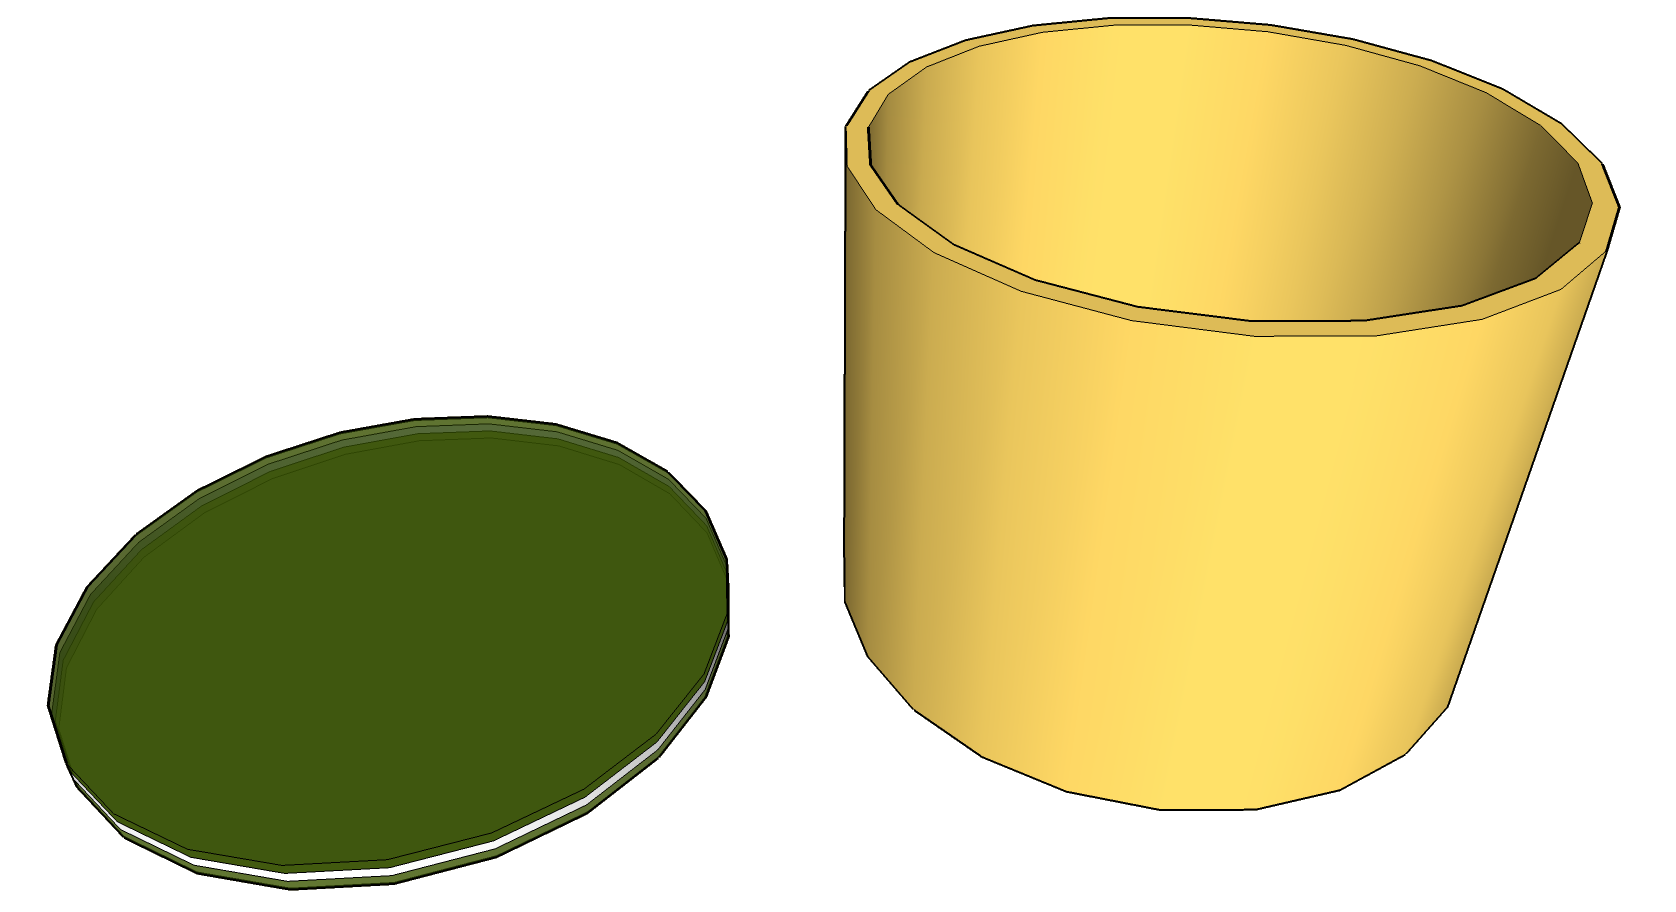
\includegraphics[width=0.838\textwidth,height=0.456\textwidth]{../images/form_factor/anisotropic/localplanar.png}
\end{center}
\caption{for local planar particles the cross section dimension is much smaller then the
radius of curvature of the particle}
\label{fig:localplanar}
\end{figure}

Several cross-section profiles for local planar objects have been implemented,
like a homogeneous cross-section,
cross-section with two infinitely thin plates,
layered centro-symmetric cross-section,
bilayer with a Gaussian scattering length density profile,
layer with Gaussian chains attached to the surface.
These form factors are supposed to be combined with a shape factor for
local planar objects which are implemented as structure  plugins
under "\texttt{by plugin|anisotropic obj.|P'Q): local planar
obj.}".

\clearpage

\subsubsection{Pcs(Q) for a homogeneous cross-section}
\label{plugin:Pcs:homogeneousXS} ~\\

\begin{figure}[htb]
\begin{center}
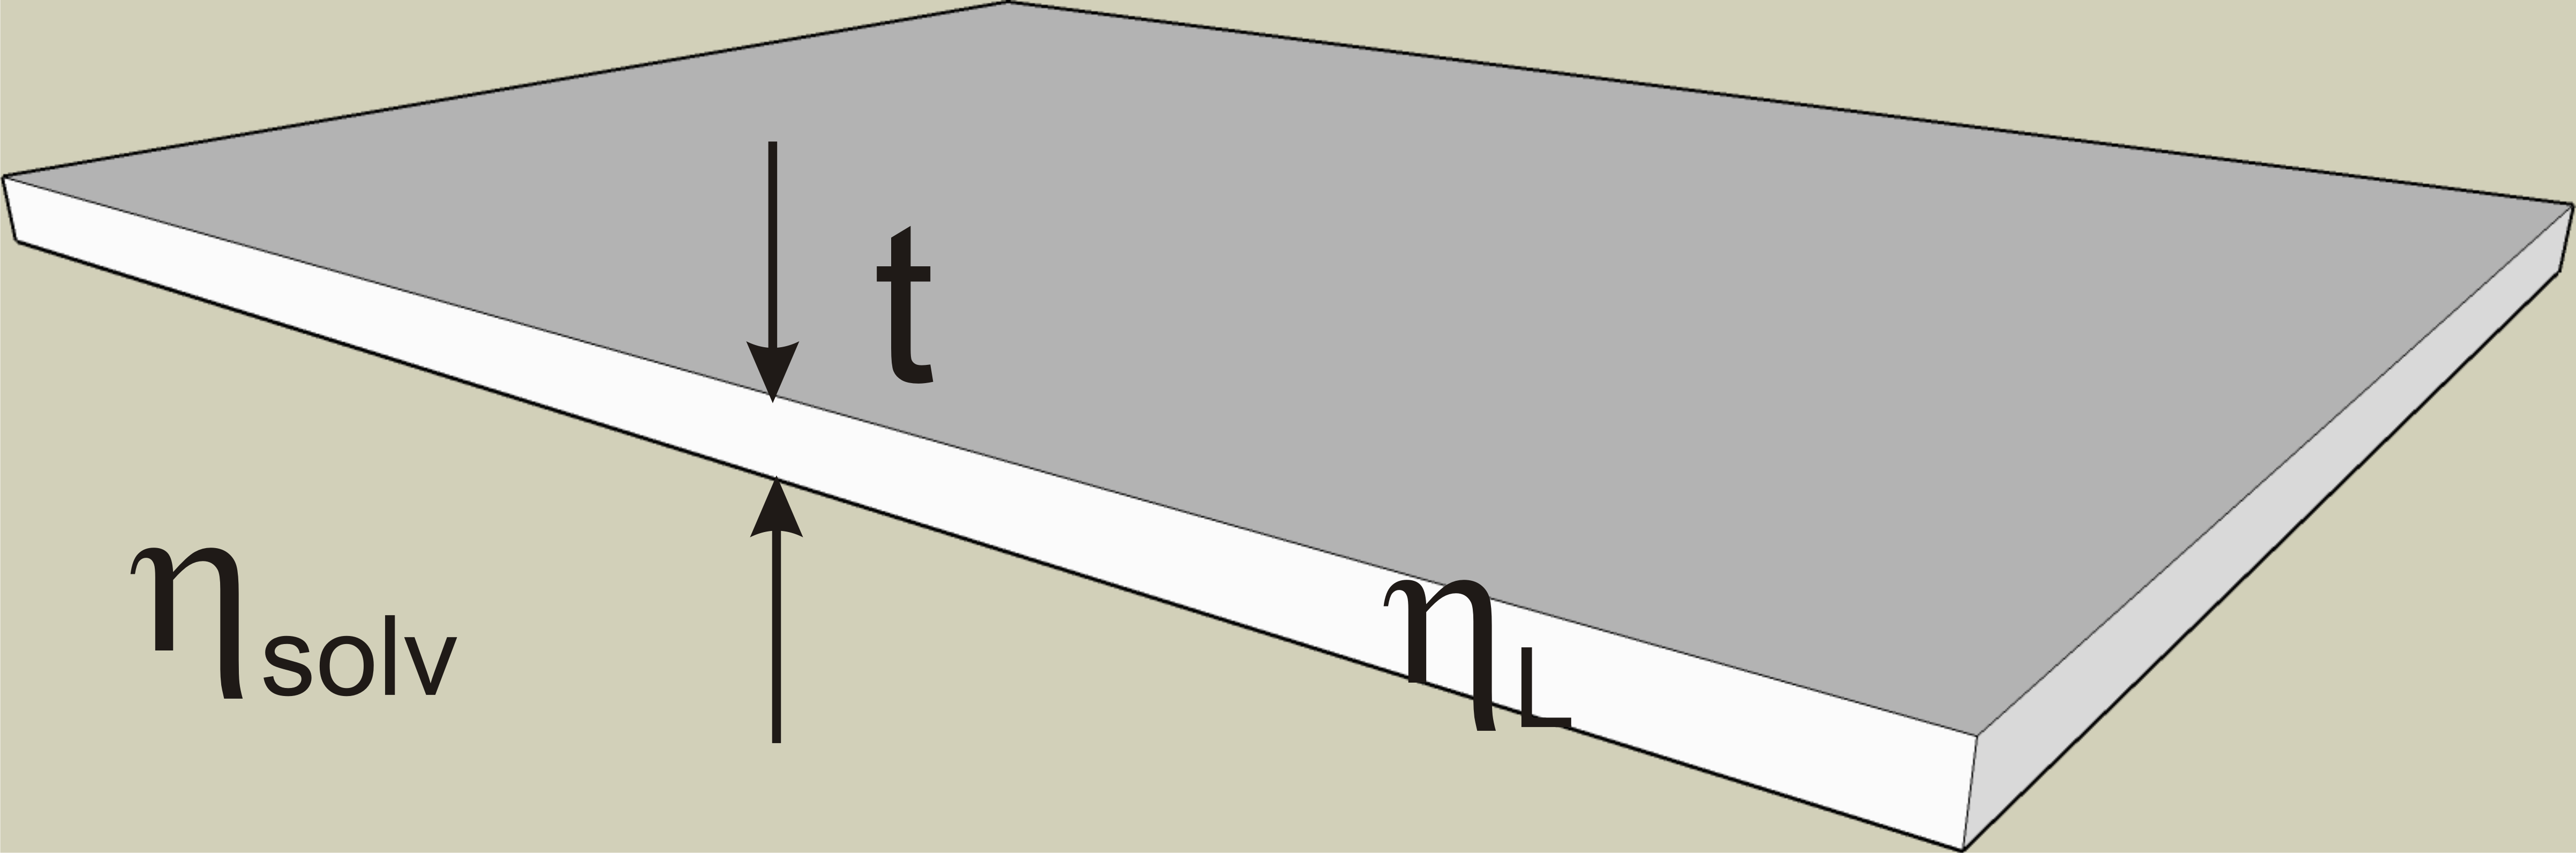
\includegraphics[width=0.802\textwidth,height=0.265\textwidth]{../images/form_factor/anisotropic/Pcs_homogeneousXS_txt.png}
\end{center}
\caption{Plane with a homogeneous cross-section of thickness $t$.}
\label{fig:homogeneousXS}
\end{figure}

This cross-section form factor describes the scattering of a layer with homogeneous
scattering length density $\eta_L$ in a matrix of a scattering length density $\eta_{solv}$.
The thickness can have a distribution described by a log-normal distribution according to eq.\ \ref{eq:LogNormal}.

\begin{align}
P_\text{cs}(Q,\sigma_{t},t) = \int_0^\infty \textrm{LogNorm}(x,1,\sigma_{t},1,t)
    \left[ \left(\eta_L-\eta_\textrm{solv}\right) x \frac{\sin(Qx/2)}{Qx/2} \right]^2\textrm{d}x
\end{align}

\noindent
\textbf{Input parameters for \texttt{Pcs:homogeneousPlate}:}
\begin{description}
    \item[\texttt{t}] most probable layer thickness $t$
    \item[\texttt{sigm\_t}] width $\sigma_t$ of thickness distribution (LogNorm)
    \item[\texttt{dummy}] unused disabled parameter
    \item[\texttt{dummy}] unused disabled parameter
    \item[\texttt{dummy}] unused disabled parameter
    \item[\texttt{dummy}] unused disabled parameter
    \item[\texttt{eta\_l}] scattering length density of layer $\eta_L$
    \item[\texttt{eta\_solv}] scattering length density of solvent $\eta_{solv}$
\end{description}

\noindent
\textbf{Note}
\begin{itemize}
  \item This form factor is supposed to be combined with a shape factor for
local planar objects which are implemented as structure  plugins
under "\texttt{by plugin|anisotropic obj.|P'Q): local planar
obj.}".
\item As the form factor already have the width distribution included one normally uses in \SASfit as a size distribution
the \texttt{Delta}-distribution.
\end{itemize}

\begin{figure}[htb]
\begin{center}
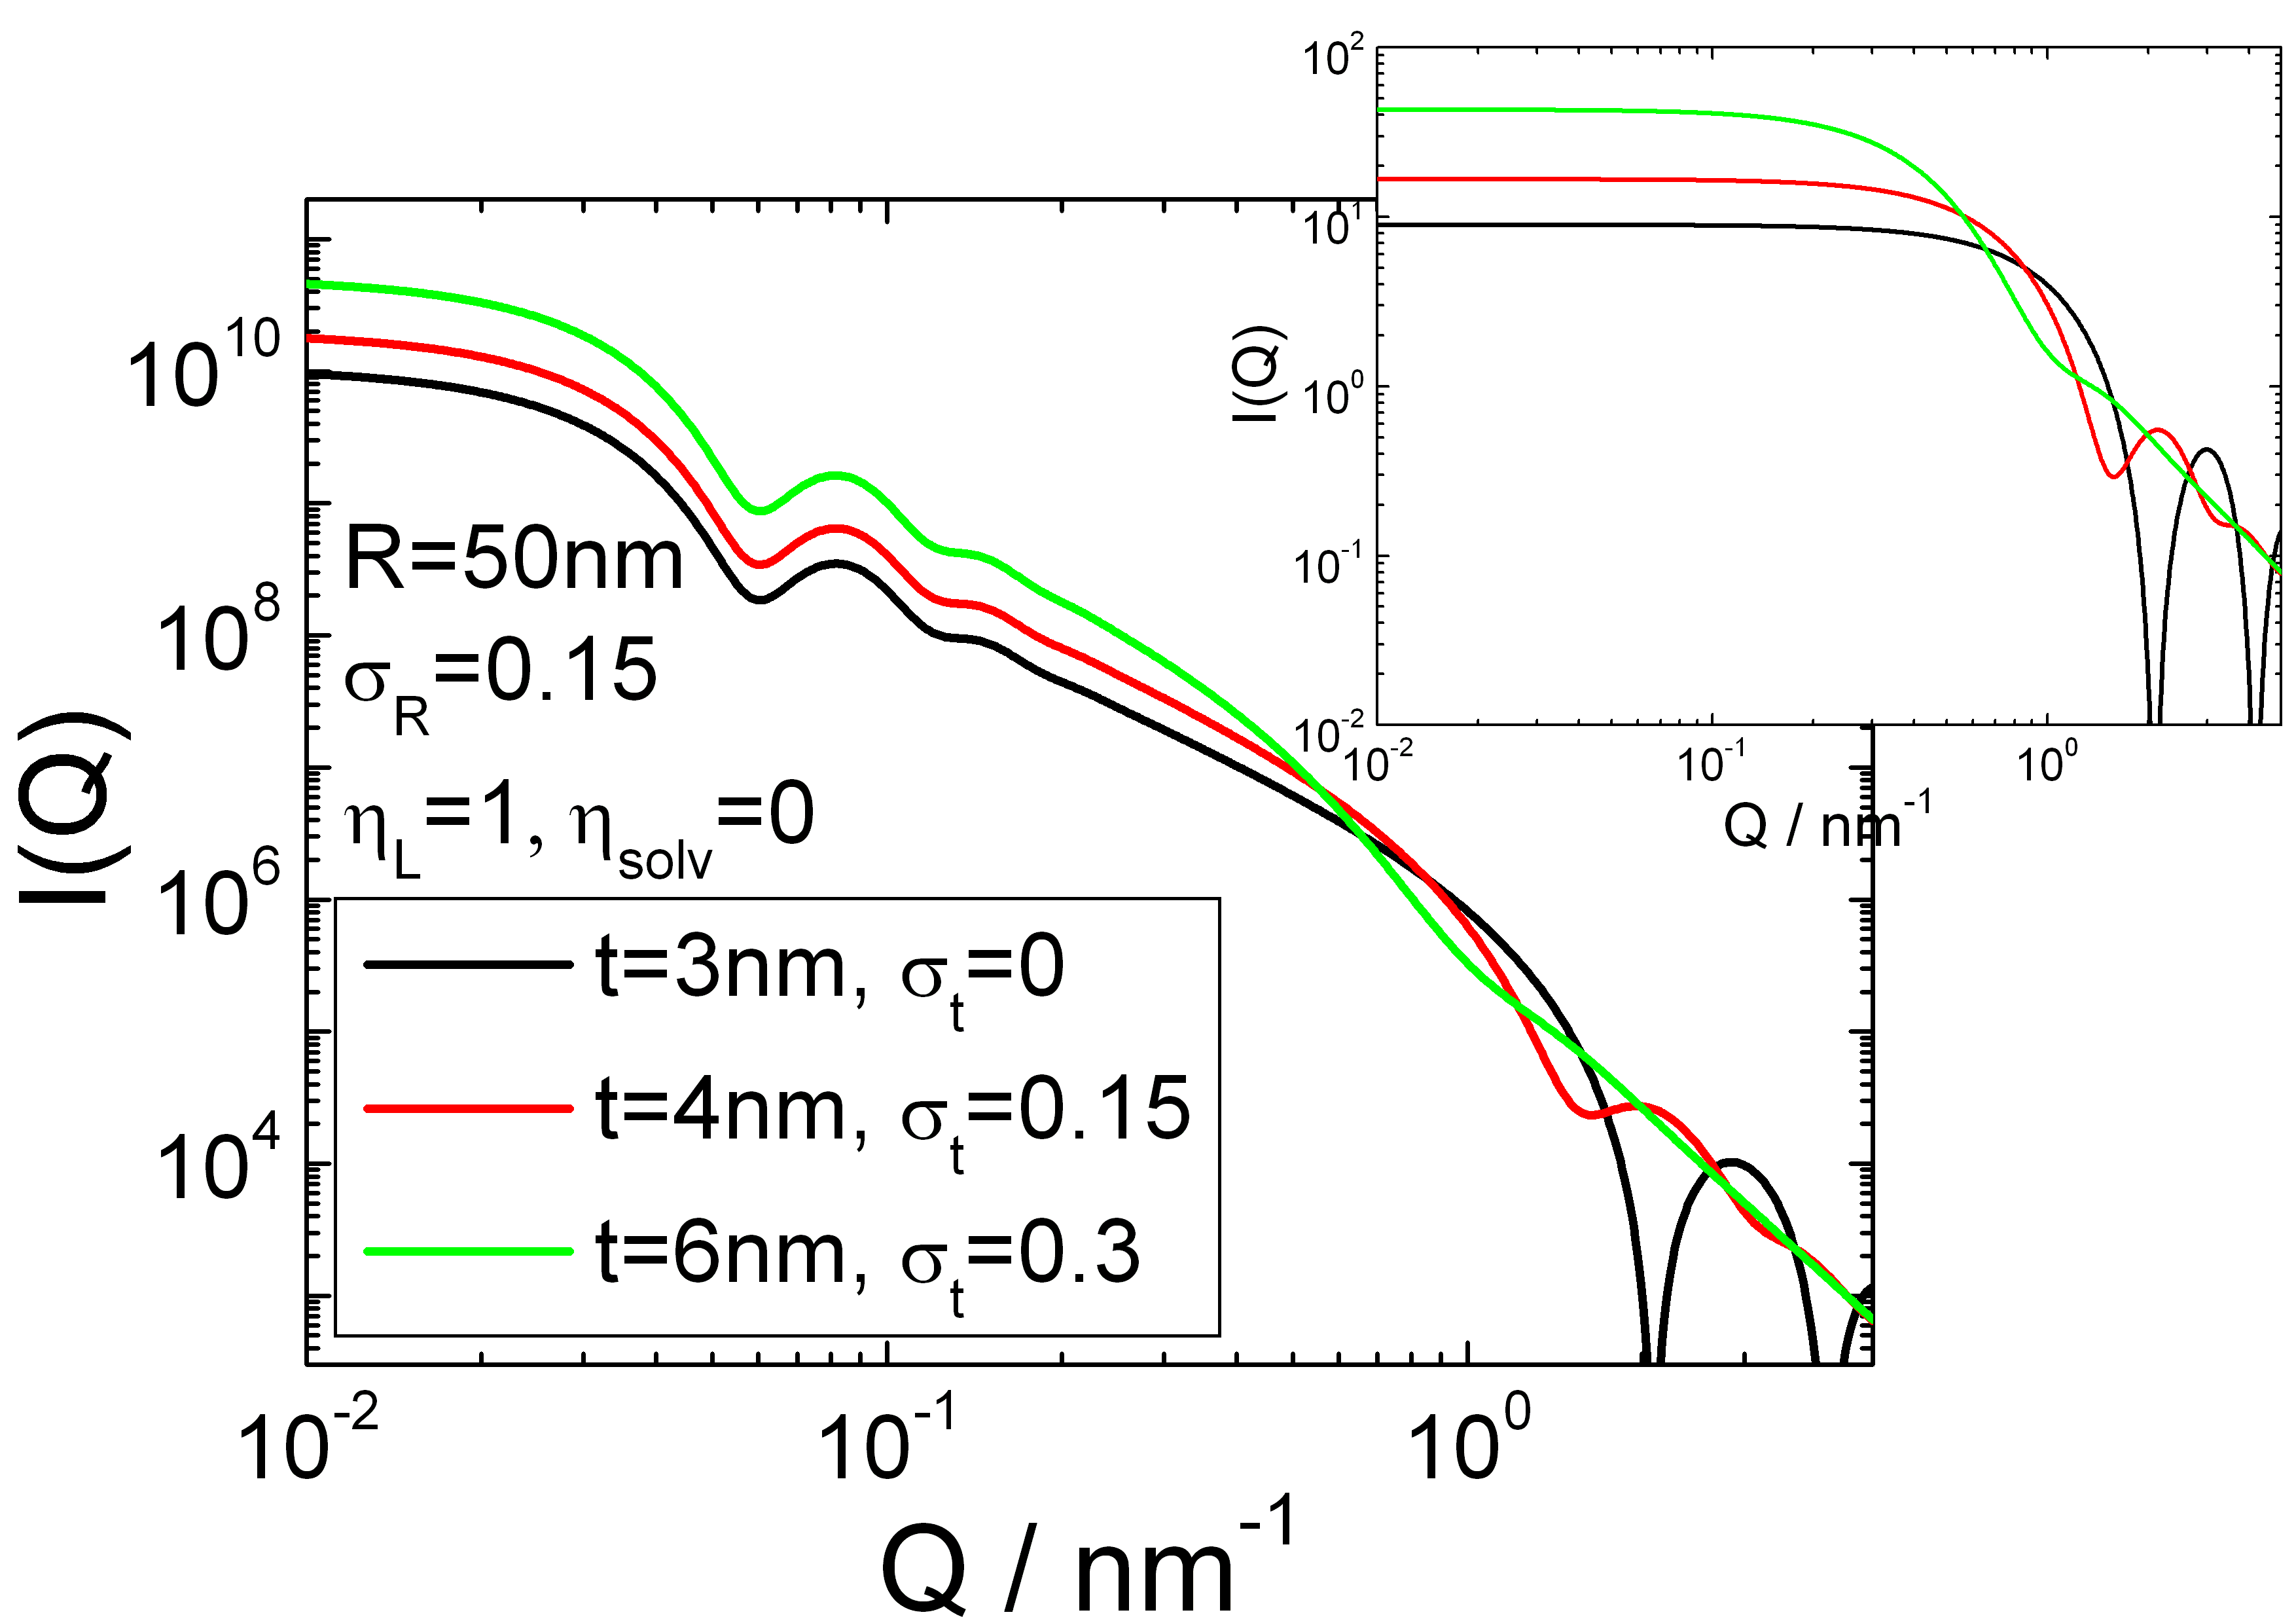
\includegraphics[width=0.8\textwidth,height=0.55\textwidth]{../images/form_factor/anisotropic/localplanarIQ.png}
\end{center}
\caption{Scattering curve for the form factor "\texttt{Pcs:homogeneousPlate}" only (insert) and
in combination with a structure factor "\texttt{P'(Q): Thin Spherical Shell}".}
\label{fig_IQ:homogeneousXS}
\end{figure}

\clearpage
\subsubsection{Pcs(Q) for two infinitely thin parallel layers} ~\\
\label{plugin:Pcs:TwoInfinitelyThinLayers}

\begin{figure}[htb]
\begin{center}
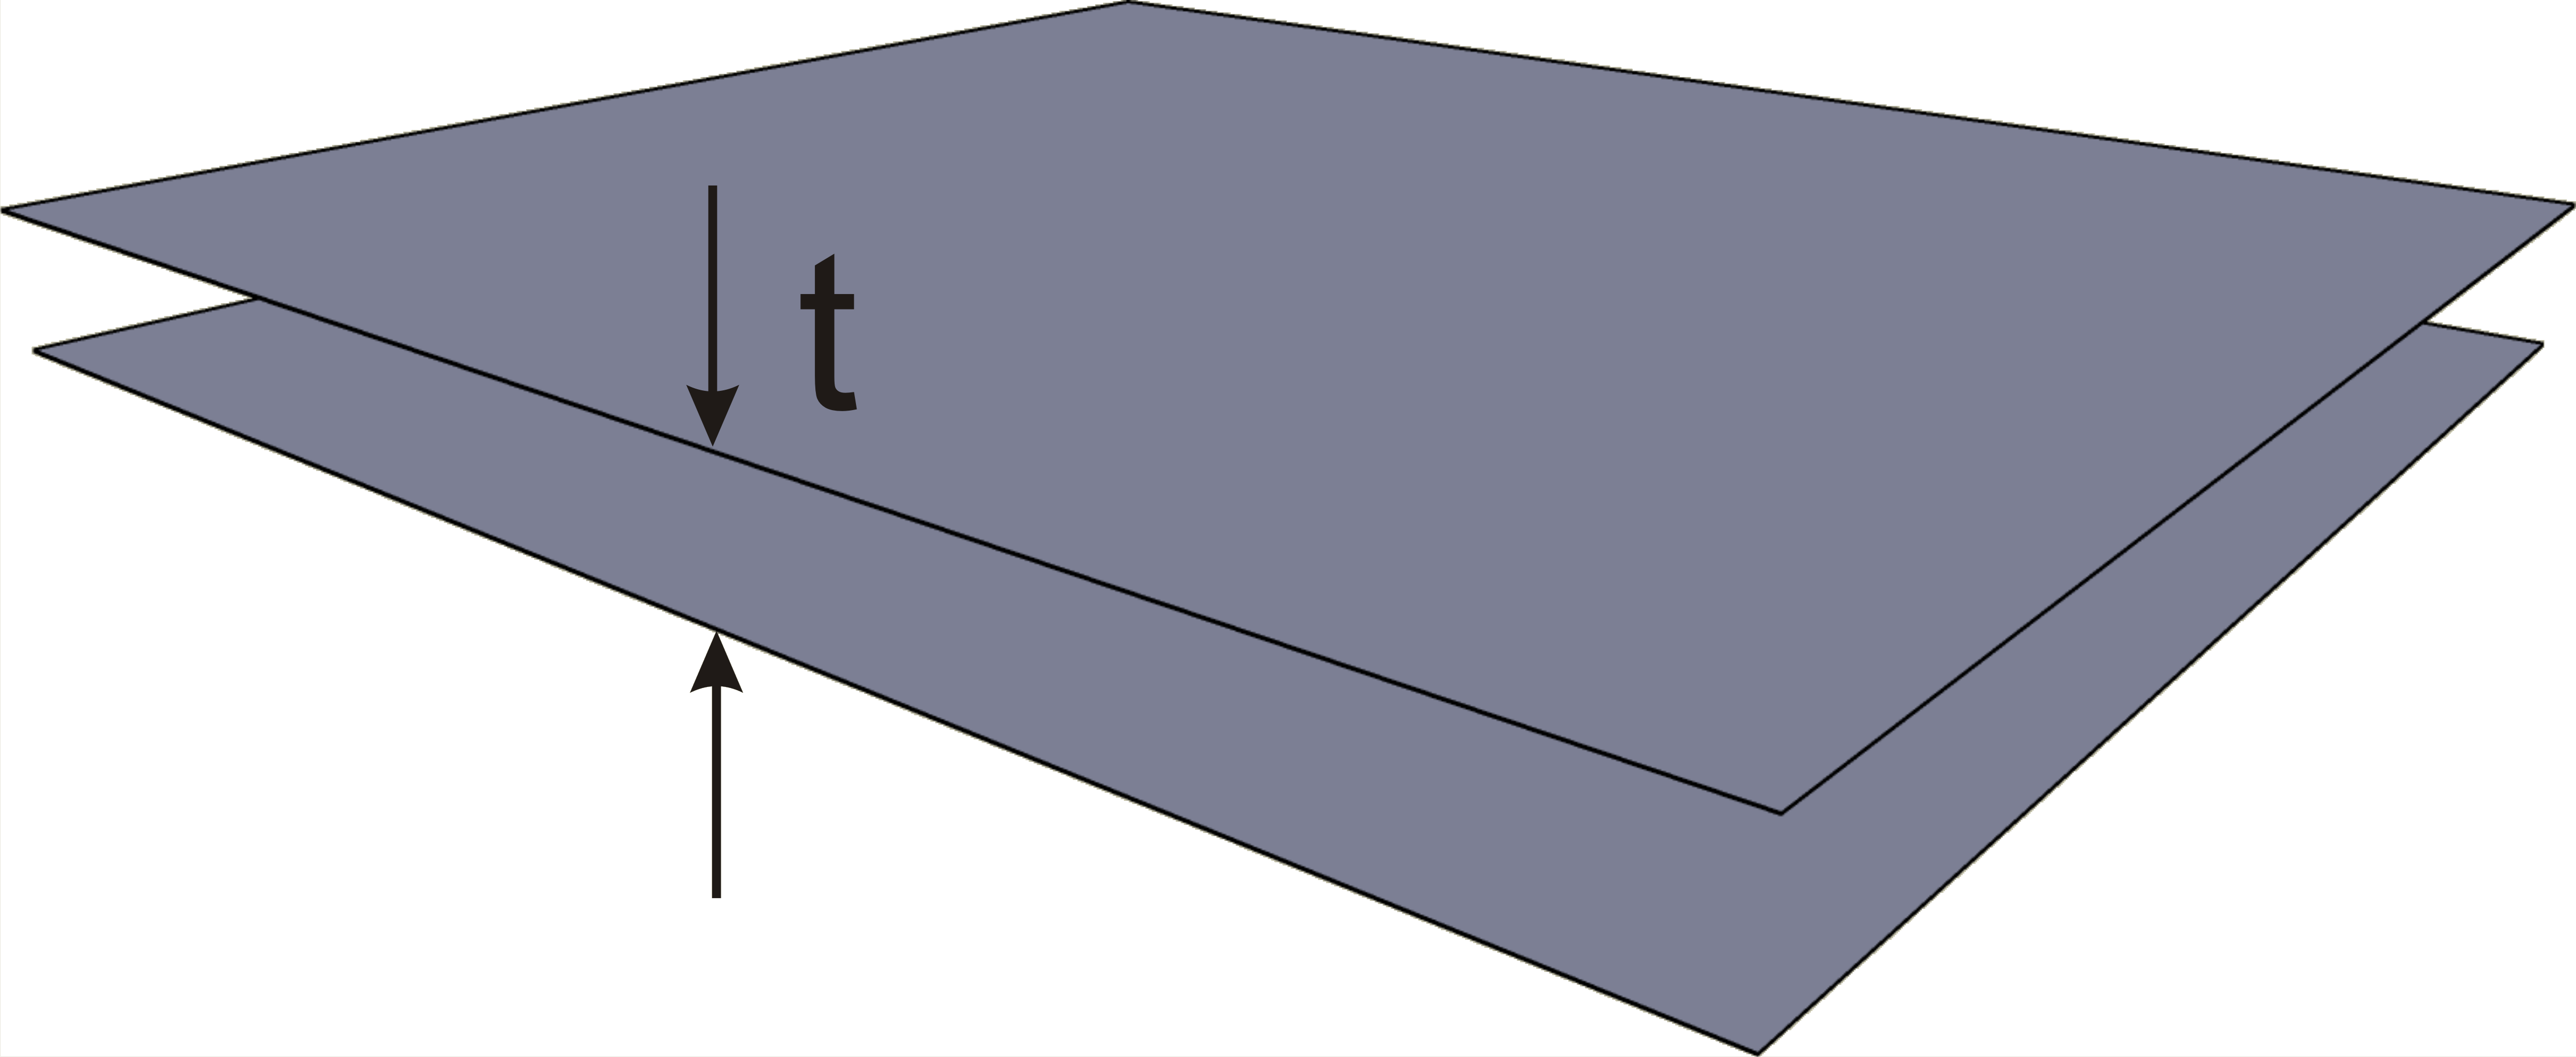
\includegraphics[width=0.8\textwidth,height=0.328\textwidth]{../images/form_factor/anisotropic/planar2thin_txt.png}
\end{center}
\caption{Two infinitely thin parallel layers separated by a distance $t$.}
\label{fig:Pcs:TwoInfinitelyThinLayers}
\end{figure}

This cross-section form factor describes the scattering of two infinitely thin parallel layers.
The separation distance can have a distribution described by a log-normal distribution according
to eq.\ \ref{eq:LogNormal}.

\begin{align}
P_\text{cs}(Q,\sigma_{T},T) = \int_0^\infty \textrm{LogNorm}(x,1,\sigma_{T},1,T) \cos^2(Qx/2) \, \textrm{d}x
\end{align}

\noindent
\textbf{Input parameters for \texttt{Pcs:TwoInfinitelyThinLayers}:}
\begin{description}
    \item[\texttt{t}] most probable layer separation $t$
    \item[\texttt{sigm\_t}] width $\sigma_t$ of separation distribution (LogNorm)
\end{description}

\noindent
\textbf{Note}
\begin{itemize}
  \item This form factor is supposed to be combined with a shape factor for
local planar objects which are implemented as structure  plugins
under "\texttt{by plugin|anisotropic obj.|P'Q): local planar
obj.}".
\item As the form factor already have the width distribution included one normally uses in \SASfit as a size distribution
the \texttt{Delta}-distribution.
\end{itemize}

\begin{figure}[htb]
\begin{center}
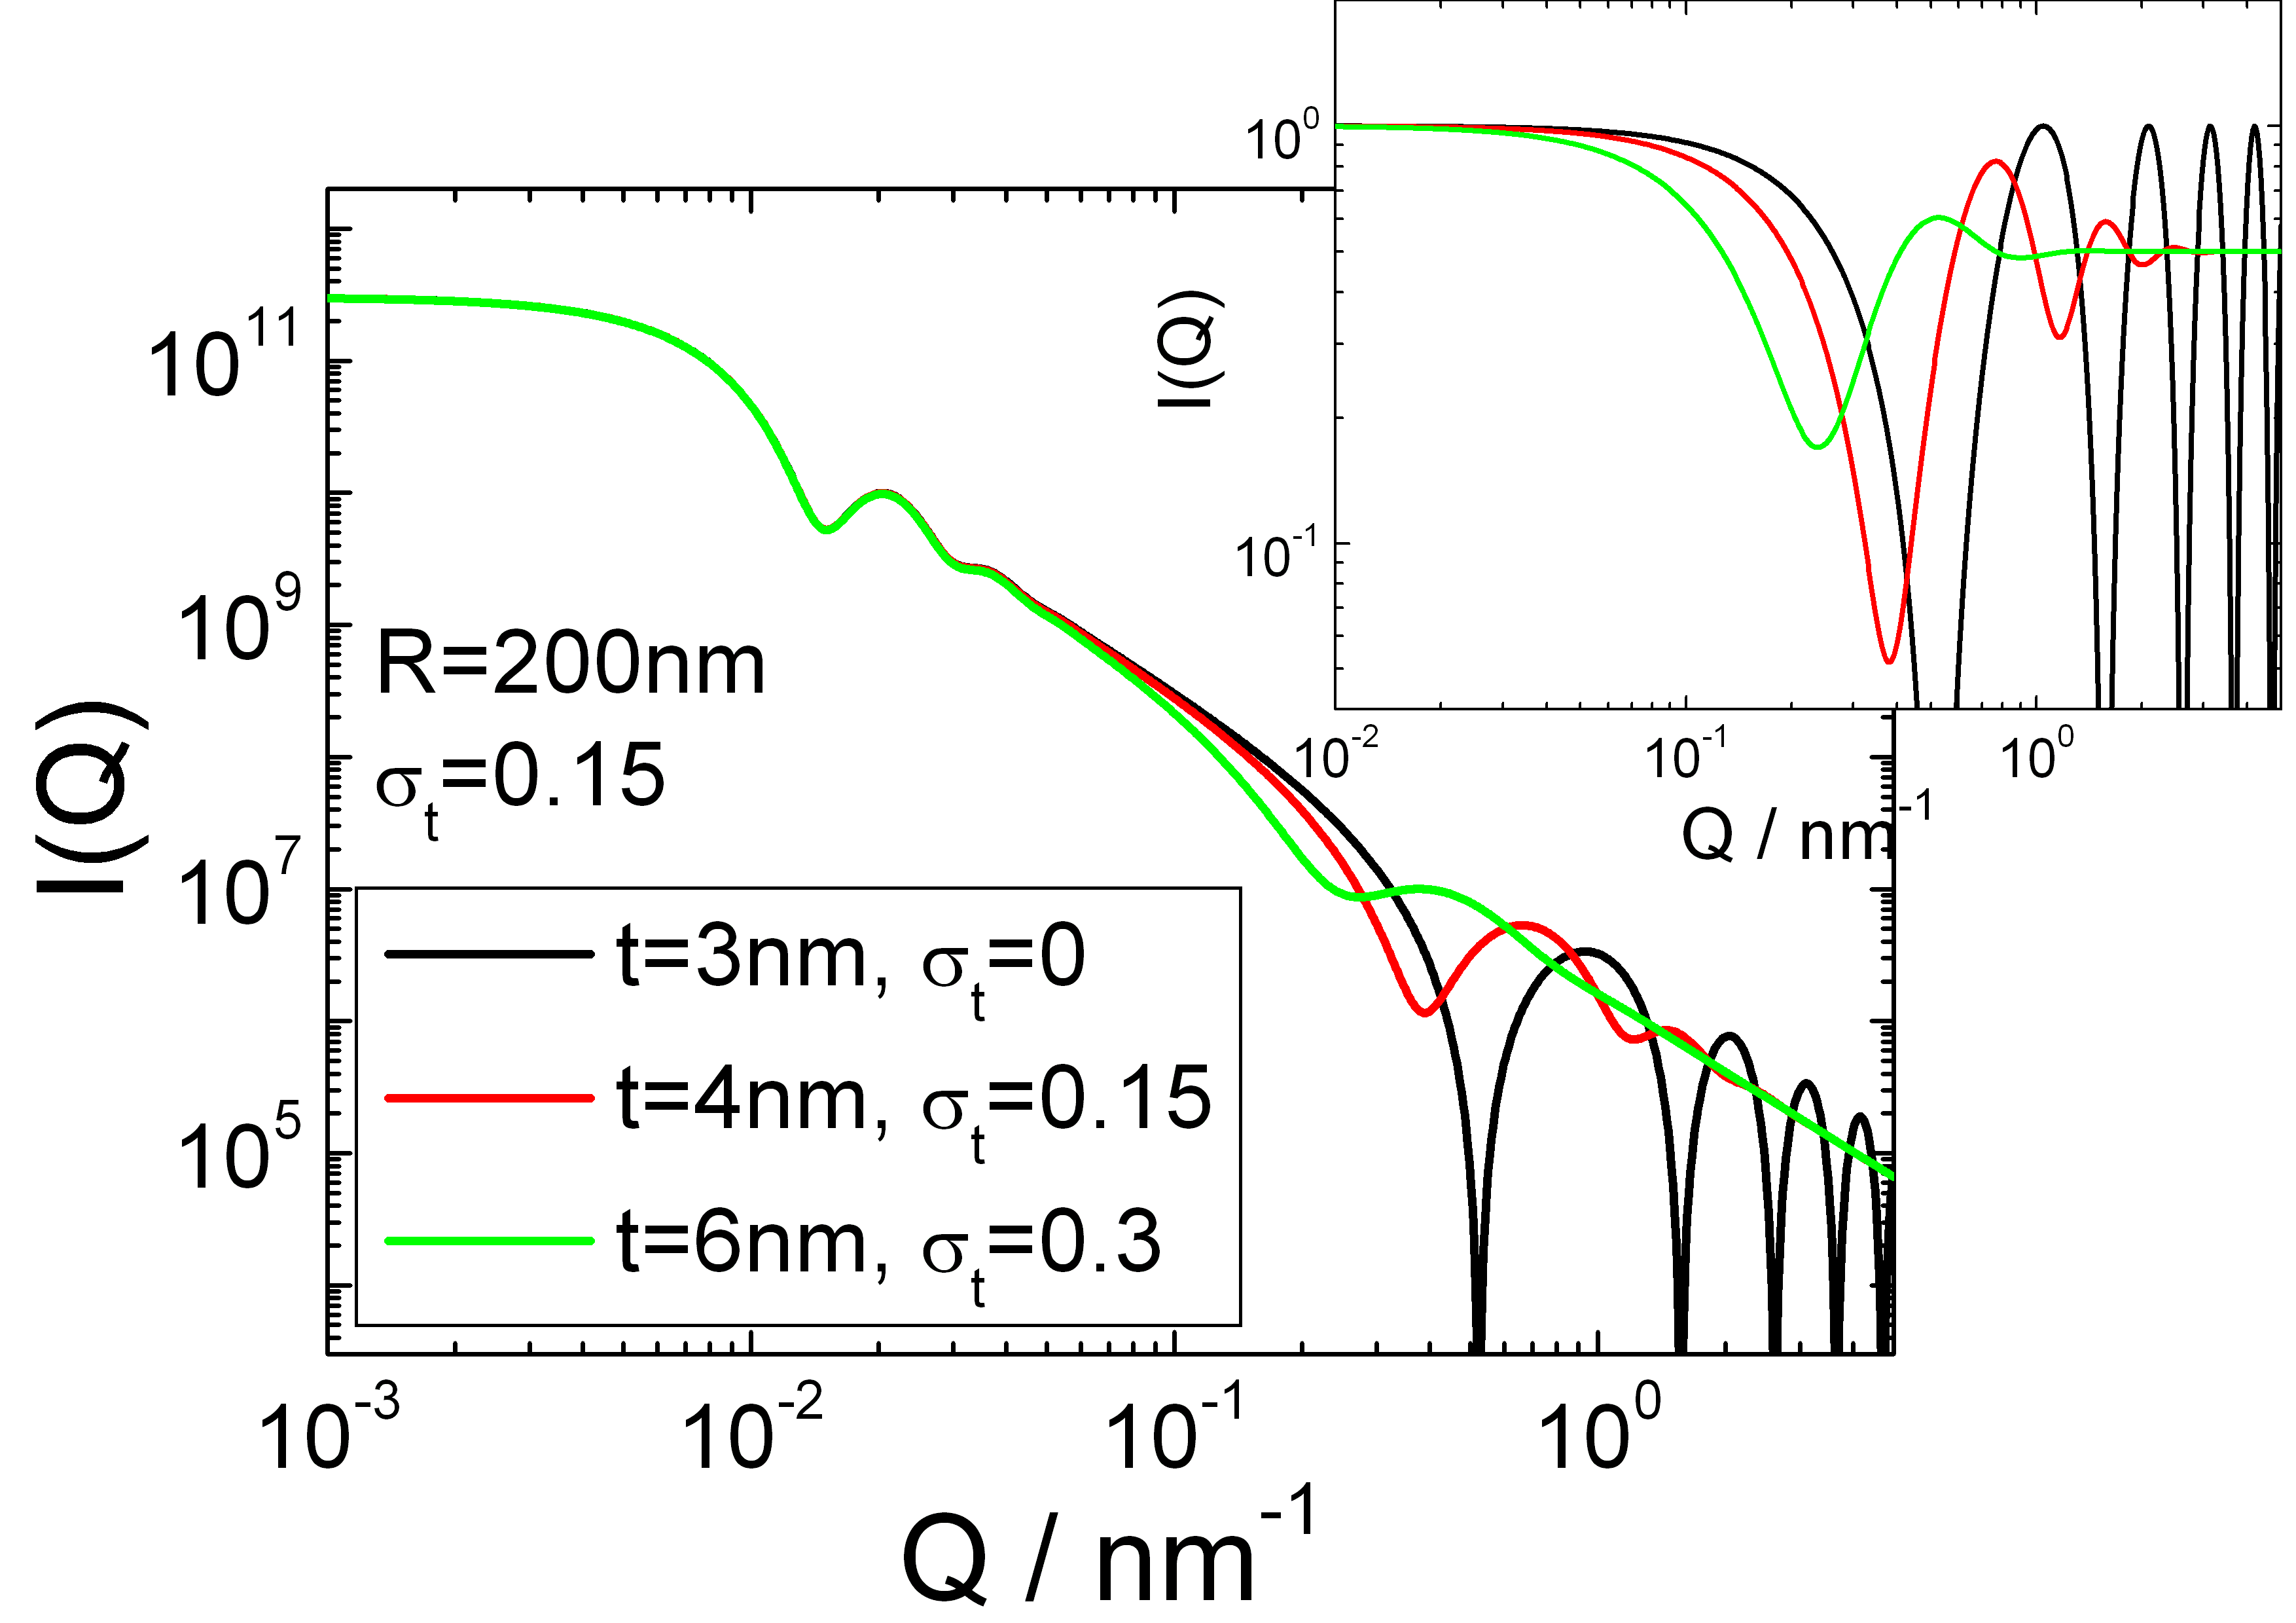
\includegraphics[width=0.8\textwidth,height=0.55\textwidth]{../images/form_factor/anisotropic/planar2thinIQ.png}
\end{center}
\caption{Scattering curve for the form factor "\texttt{Pcs:TwoInfinitelyThinLayers}" only (insert) and
in combination with a structure factor "\texttt{P'(Q): Thin Spherical Shell}".}
\label{fig_IQ:Pcs:TwoInfinitelyThinLayers}
\end{figure}


\clearpage
\subsubsection{Pcs(Q) for a layered centro symmetric cross-section structure} ~\\
\label{plugin:Pcs:LayeredCentroSymmetricCrossSectionStructure}

\begin{figure}[htb]
\begin{center}
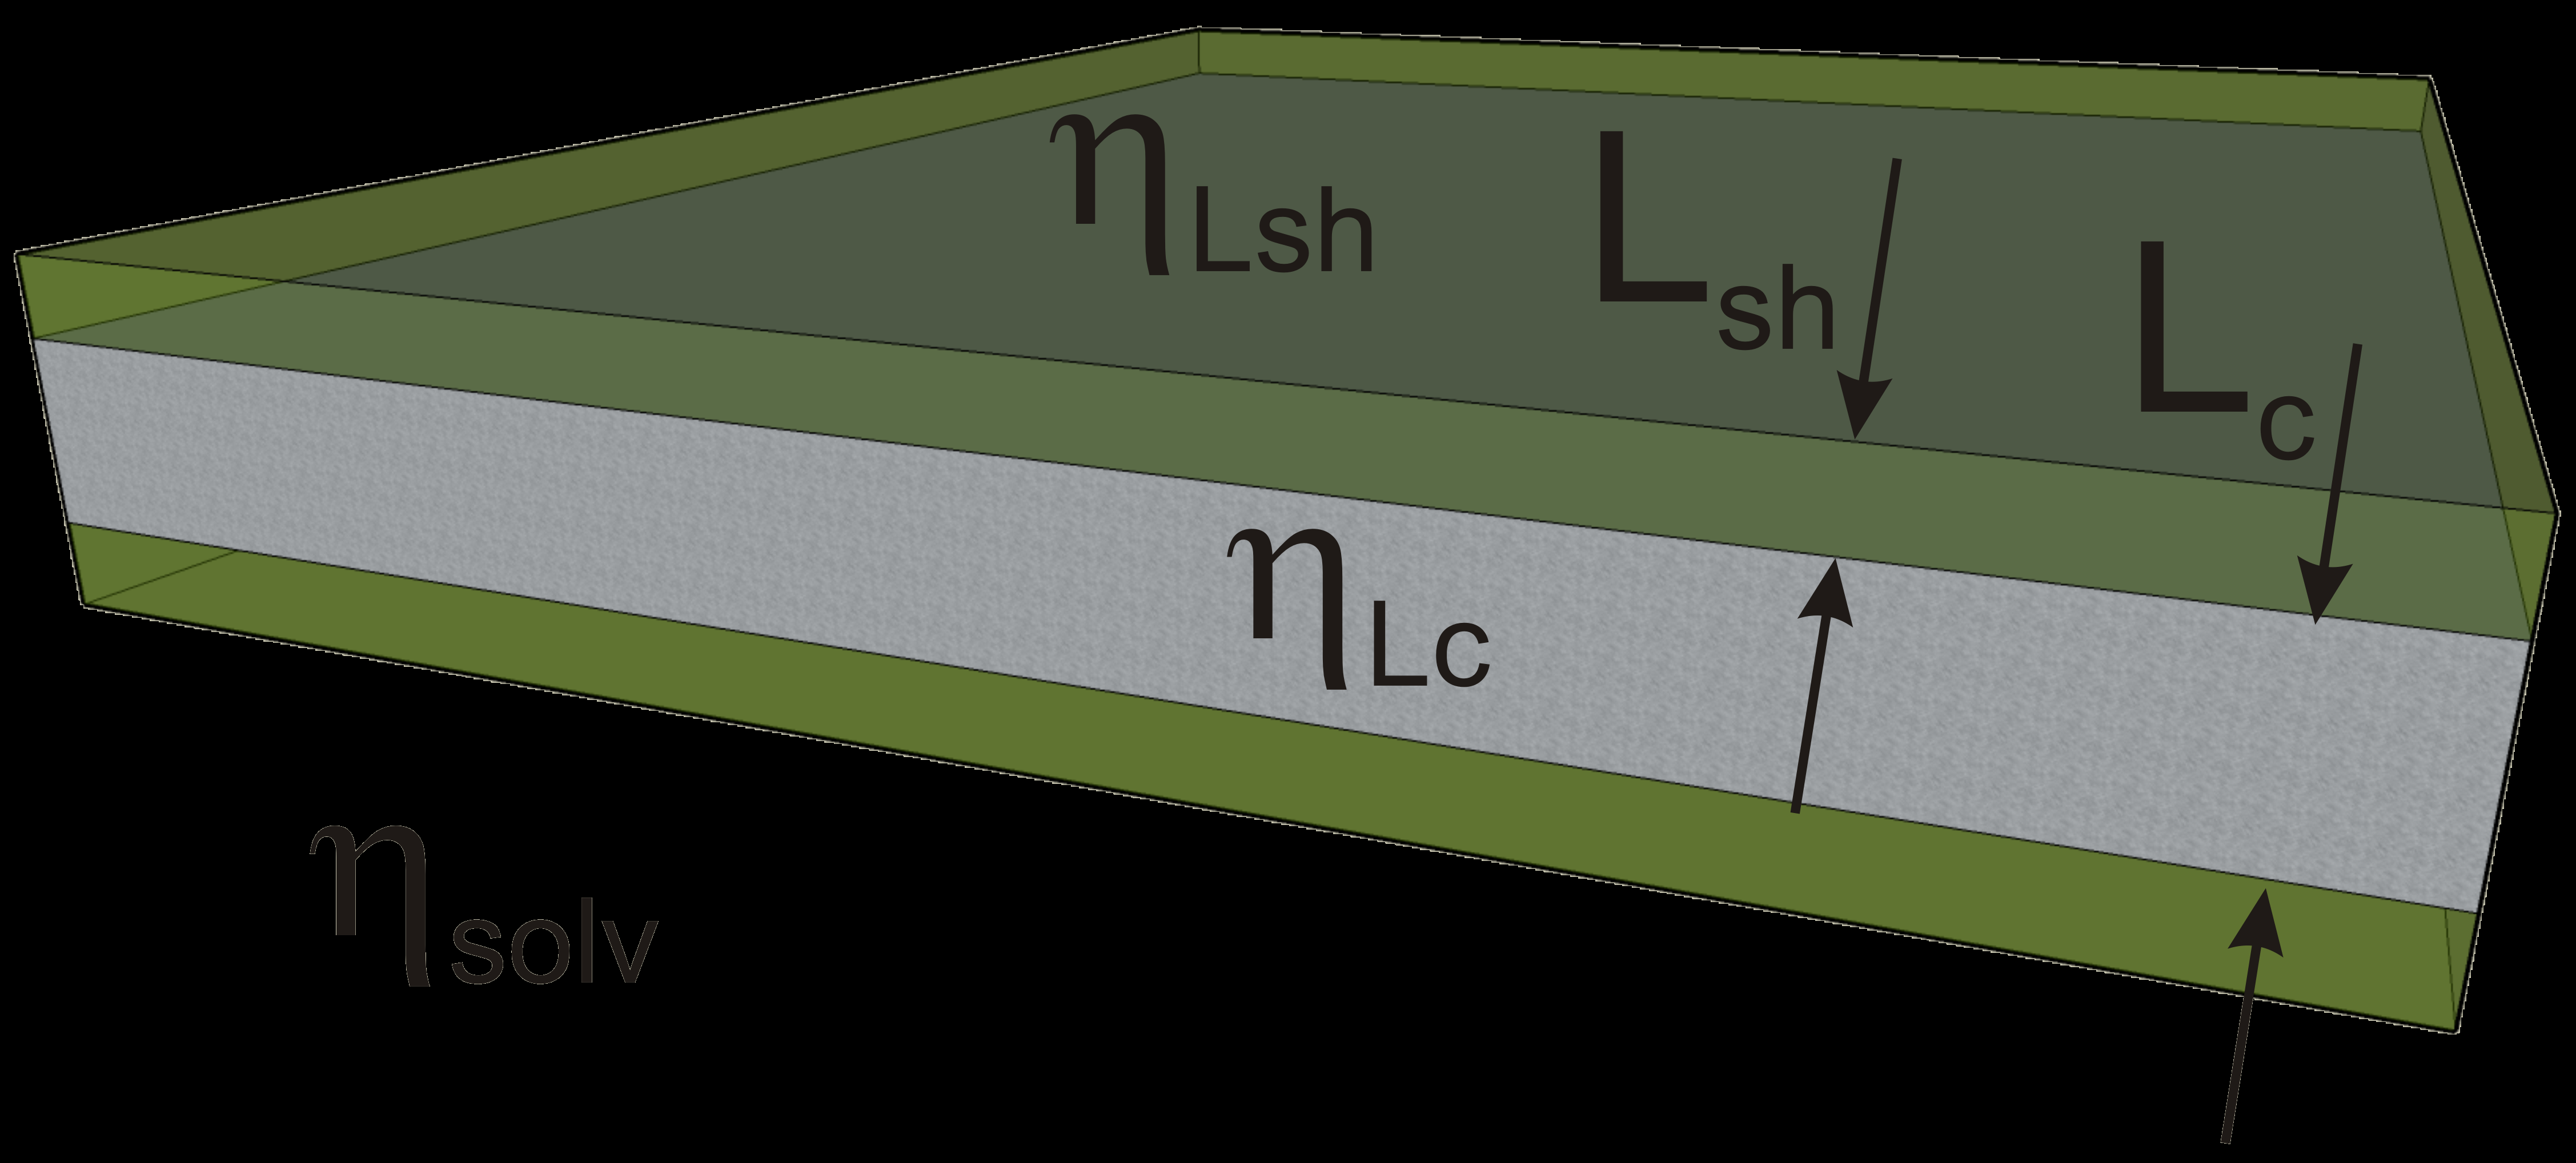
\includegraphics[width=0.8\textwidth,height=0.361\textwidth]{../images/form_factor/anisotropic/planar2centrosymm_txt.png}
\end{center}
\caption{Two layered centro symmetric structure with a core thickness of $L_\textrm{c}$ and an outer layer thickness
$L_{L_\textrm{sh}}$. The corresponding scattering length densities of the core, the shell layer and the solvent are
$L_{L_\textrm{c}}$, $L_{L_\textrm{sh}}$, and $L_{L_\textrm{solv}}$.}
\label{fig:Pcs:TwoInfinitelyThinLayers}
\end{figure}

This cross-section form factor describes the scattering of a layered centro symmetric cross-section structure.
Both the core thickness as well as the shell thickness can have a distribution described by a log-normal distribution as defined in eq.\ \ref{eq:LogNormal}.

\begin{multline}
P_\text{cs}(Q,\sigma_{L_\textrm{c}},L_\textrm{c},\sigma_{L_\textrm{sh}},L_\textrm{sh},\eta_{L_\textrm{c}},\eta_{L_\textrm{sh}},\eta_\textrm{sol}) = \\
\int_0^\infty \textrm{LogNorm}(v,1,\sigma_{L_\textrm{c}},1,L_\textrm{c})
\int_0^\infty \textrm{LogNorm}(u,1,\sigma_{L_\textrm{sh}},1,L_\textrm{sh}) \\
     \Bigg[ \frac{(\eta_{L_\textrm{sh}}-\eta_\textrm{solv})(v+2u) \sin\left(Q\frac{v+2u}{2}\right)}{Q\frac{v+2u}{2}}
          -\frac{(\eta_{L_\textrm{sh}}-\eta_{L_\textrm{c}})  v   \sin\left(Q \frac{v}{2}\right)}{Q \frac{v}{2}}
    \Bigg]^2 \,
\textrm{d}u \, \textrm{d}v
\end{multline}

\noindent
\textbf{Input parameters for \texttt{Pcs:LayeredCentroSymmetricXS}:}
\begin{description}
    \item[\texttt{L\_c}] most probable layer separation $L_\textrm{c}$
    \item[\texttt{sigm\_Lc}] width $\sigma_{L_\textrm{c}}$ of core thickness distribution (LogNorm)
    \item[\texttt{L\_sh}] most probable shell thickness $L_\textrm{sh}$
    \item[\texttt{sigm\_Lsh}] width $\sigma_{L_\textrm{c}}$ of shell thickness distribution (LogNorm)
    \item[\texttt{dummy}] unused disabled parameter
    \item[\texttt{dummy}] unused disabled parameter
    \item[\texttt{eta\_Lc}] scattering length density of core layer $\eta_{L_\textrm{c}}$
    \item[\texttt{eta\_Lsh}] scattering length density of shell layer $\eta_{L_\textrm{sh}}$
    \item[\texttt{eta\_solv}] scattering length density of solvent $\eta_{solv}$
\end{description}

\noindent
\textbf{Note}
\begin{itemize}
  \item This form factor is supposed to be combined with a shape factor for
local planar objects which are implemented as structure  plugins
under "\texttt{by plugin|anisotropic obj.|P'Q): local planar
obj.}".
\item As the form factor already have the width distribution included one normally uses in \SASfit as a size distribution
the \texttt{Delta}-distribution.
\end{itemize}

\begin{figure}[htb]
\begin{center}
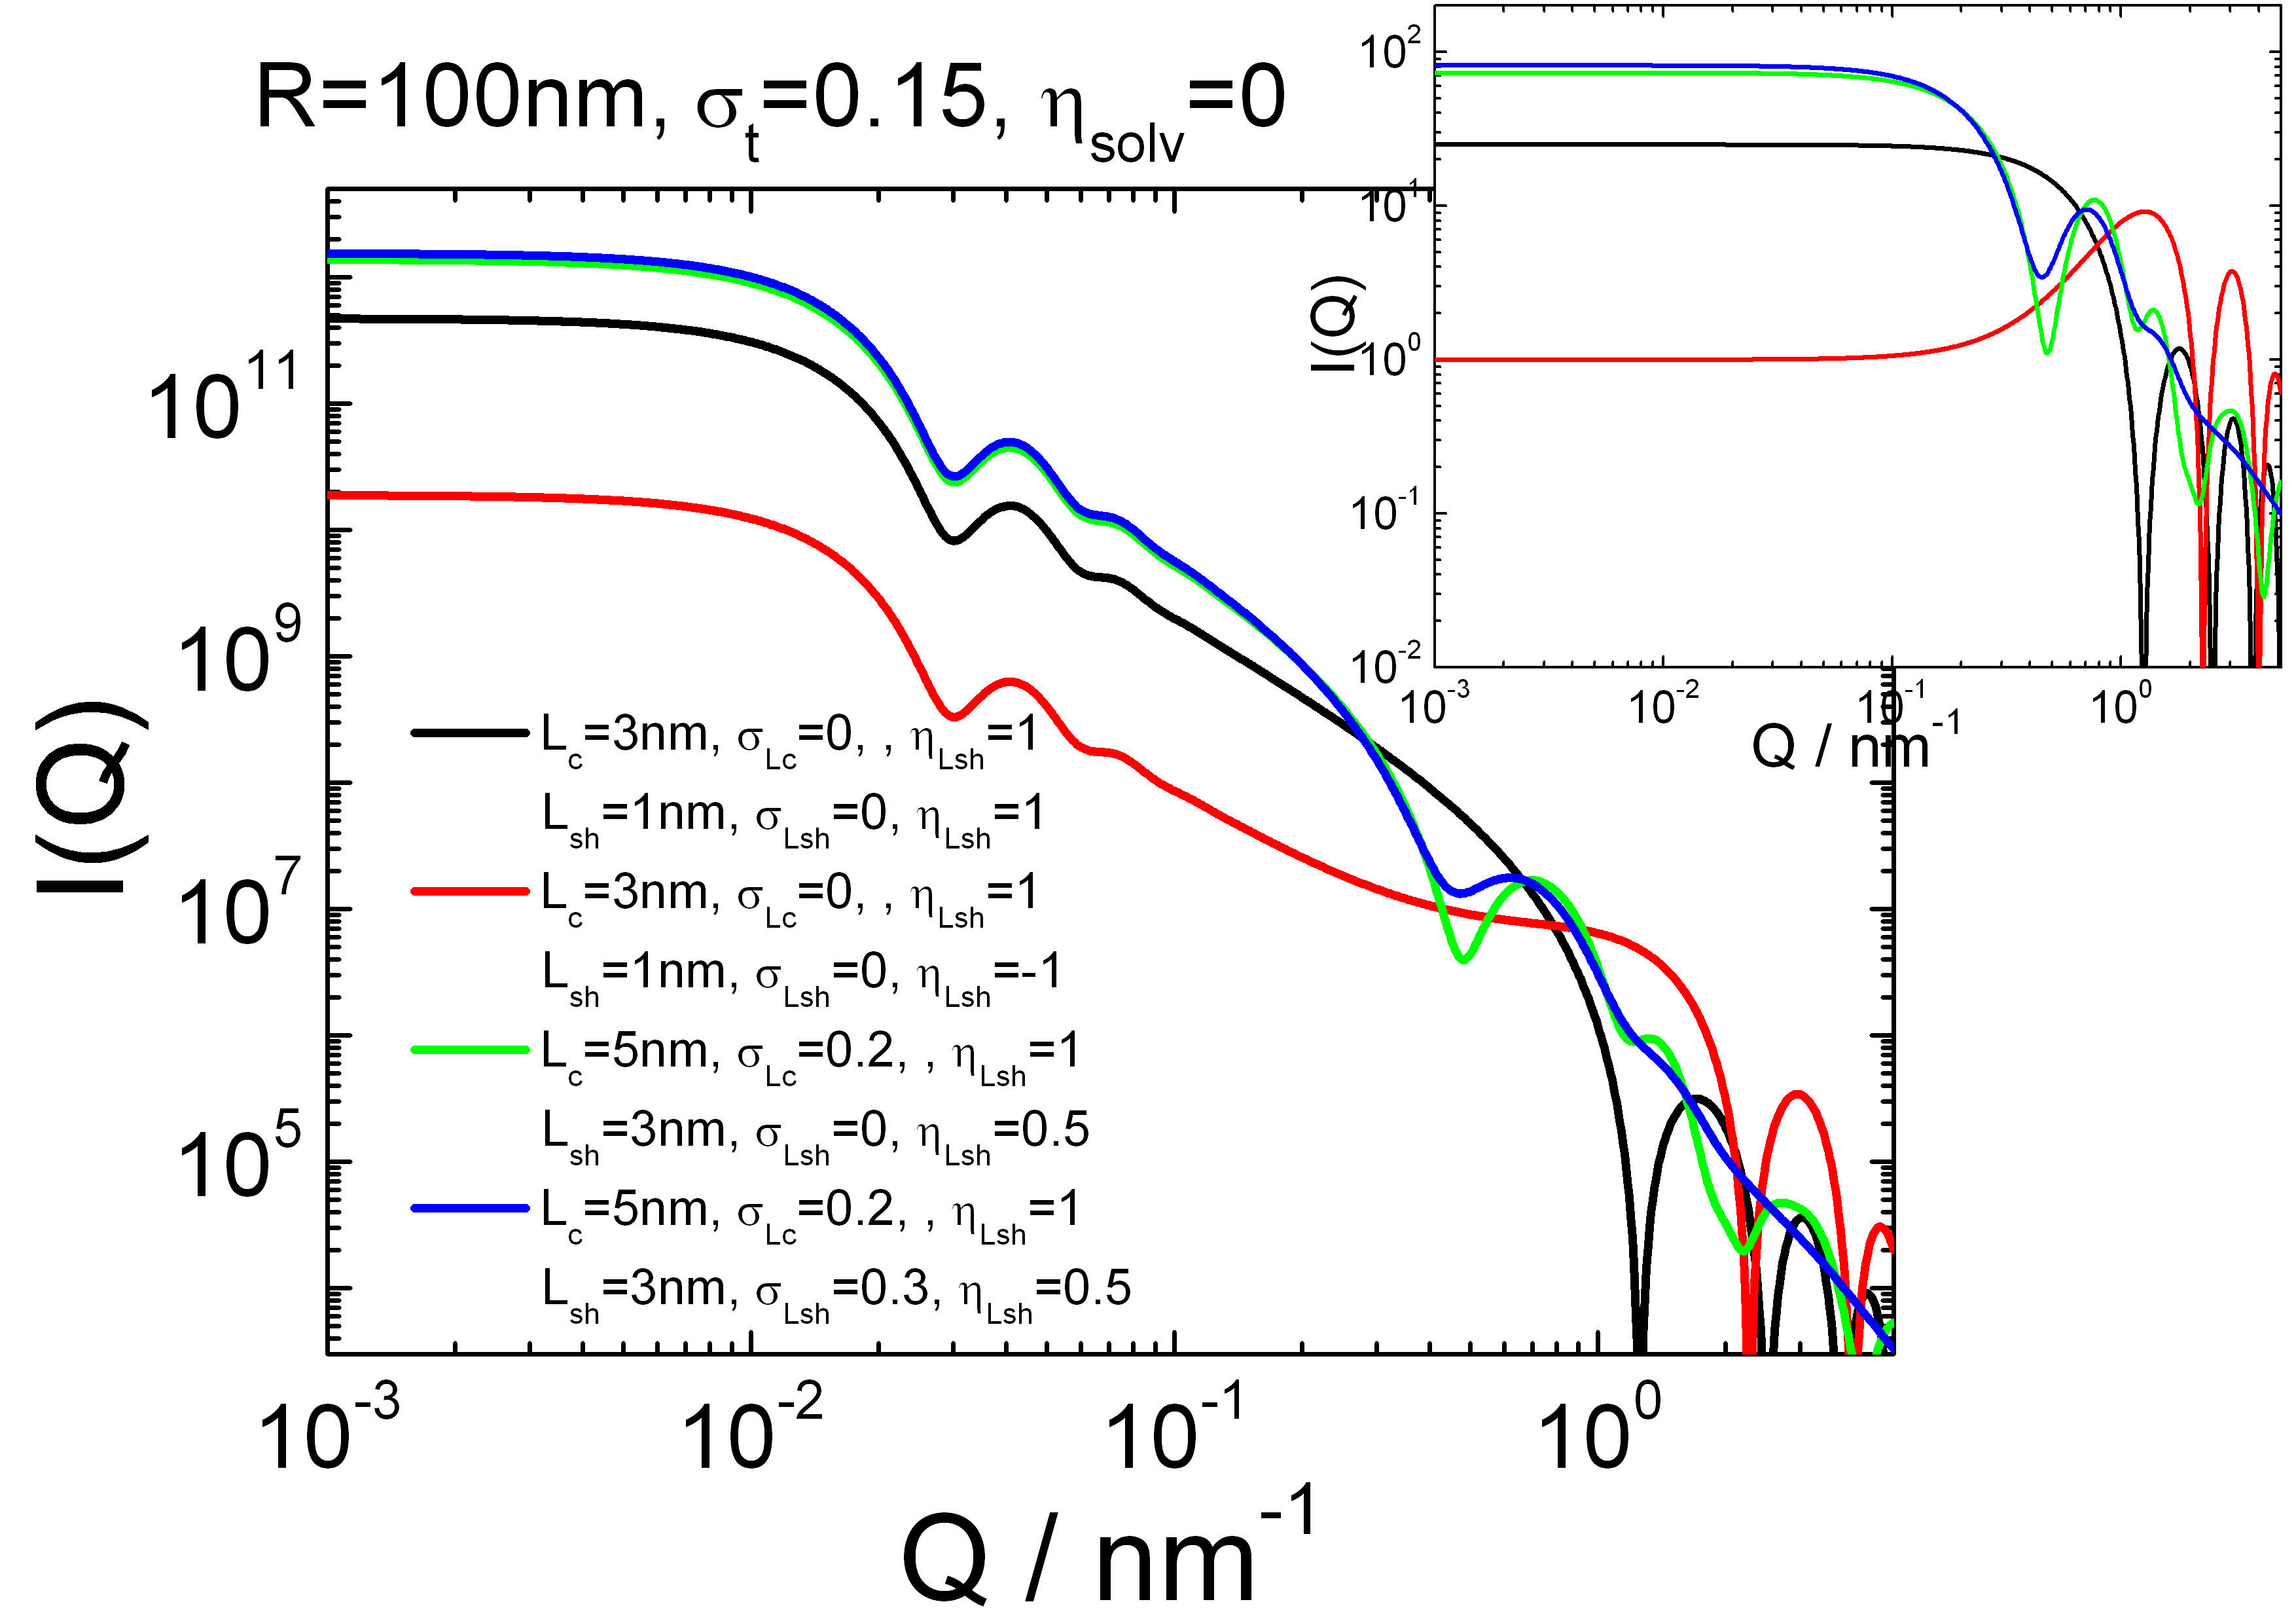
\includegraphics[width=0.8\textwidth,height=0.55\textwidth]{../images/form_factor/anisotropic/Pcs_planar2centrosymmIQ.png}
\end{center}
\caption{Scattering curve for the form factor "\texttt{Pcs:LayeredCentroSymmetricXS}" only (insert) and
in combination with a structure factor "\texttt{P'(Q): Thin Spherical Shell}".}
\label{fig:Pcs_planar2centrosymmIQ}
\end{figure}

\clearpage

\subsubsection{Pcs(Q) for  particles with Gaussian chains attached to the
surface} ~\\
\label{plugin:Pcs:GaussianChains}

\vspace{5mm}

\subsubsection{Pcs(Q) for a bilayer with density profile} ~\\
\label{plugin:Pcs:GaussianProfile}


\clearpage
\subsection{Pcs(Q) for cylindrical obj.} ~\\
\label{plugin:Pcs4cylindrical}

The cross-section form factors with cylindrical geometry are valid
when the cross-section dimension is much smaller the segment length
or Kuhn length of the local cylindrical structure.

\subsection{P'(Q) for local planar obj.} ~\\
\label{plugin:Pprime4planar}


\subsection{P'(Q) for local cylindrical obj.} ~\\
\label{plugin:Pprime4cylindrical}

\subsection{local planar  obj.} ~\\
\label{plugin:LocalPlanar)}

\subsection{local cylindrical obj.} ~\\
\label{plugin:LocalCylindrical)}

%%%%%%%%%%%%%%%%%%%%%%%%%%%%%%%%%%%%%%%%%%%%%%%%%%%%%%%%%%%%%%%%%%%%%%%%%

\clearpage
\section{JuelichCoreShell} ~\\

This model considers a dense core and original two shells
\cite{Willner2000}. Besides, it considers two different density
profiles: a parabolic and a star-like profile for the second shell.
\begin{align}
\eta_\text{shell}(r) & \propto r^{-x} \quad \text{for starlike profile $x=4/3$}\\
\eta_\text{shell}(r) & \propto 1-\left(\frac{r}{L_p}\right)^{2}
\quad \text{for parabolic profile of thickness $L_p$}
\end{align}
Model parameters:
\begin{description}
\item[$b_\text{solv}$]  scattering length density of the solvent
\item[$I_0$] forward scattering
\item[$M_\text{core}$] molecular weight of core (g/mol)
\item[$M_\text{brush}$] molecular weight brush (g/mol)
\item[$\rho_\text{core}$] mass density of core matter (g/cm$^3$)
\item[$\rho_\text{brush}$] mass density of brush matter (g/cm$^3$)
\item[$b_\text{core}$] scattering length density of core material (cm$^{-2}$)
\item[$b_\text{brush}$] scattering length density of brush material (cm$^{-2}$)
\item[$N_\text{agg}$] aggregation number (real number)
\item[$d_c^+$] extra radius of core (compared to compact)
\item[$p_{12}$] relative distribution of shell amount in
(1$^\text{st}$shell:2$^\text{nd}$shell) ($0\ldots\infty$)
\item[$d_1^+$] extra radius of first shell (compared to compact)
\item[$d_2^+$] extra radius of second shell (compared to compact)
\item[$\sigma_c$] core smearing
\item[$\sigma_1$] smearing of 1$^\text{st}$ shell
\item[$\sigma_2$] smearing of 2$^\text{nd}$ shell
\item[$x_\text{star}$] relative distribution of
parbolic:starlike profile in 2$^\text{nd}$ shell, one has to put a
very high value in order to consider only a star-like profile.
\item[$\gamma$] for star-like profile the exponent is $4/3$ and for a constant profile chose 0
\item[$L_p$] thickness of parabolic brush (must fit in 2$^\text{nd}$ shell!)
\end{description}
%parnam(16)= 'f_brush' scattering length density correction factor brush
%parnam(17)= 'f_core' scattering length density correction factor core
\begin{align}
I(Q) = %\frac{amplitu}{V_c+V_b}
\left[\Delta b_c F_c + \Delta b_b (F_1+F_2)\right]^2
\end{align}
\begin{align}
\Delta b_c &= b_\text{core} - b_\text{solv}  (1-f_\text{core}) \\
\Delta b_b &= b_\text{brush} - b_\text{solv} (1-f_\text{brush})
\end{align}
$V_c$ and $V_b$ are the core and shell bulk volumes respectively.
\\

\noindent \textbf{Mass Conservation:} \\
From the given values of the molecular weights of the two blocks and
their densities, and an assumed aggregation number $N_\text{agg}$,
the bulk volumes of the core and the shell, $V_c$ and $V_b$, can be
calculated.

\noindent \textbf{Core:}
\begin{align}
& \text{bulk core volume:} \quad          V_c = \frac{N_\text{agg} M_\text{core}}{\rho_\text{core}N_a} \\
& \text{minimal radius of core:} \quad    R_c^0 = \left(\frac{3}{4\pi} V_c\right)^{1/3} \\
& \text{effective core radius:} \quad     R_c = R_c^0 + d_c^+ \\
& \text{swollen core volume:} \quad       V_{sc} = \frac{4}{3}\pi R_c^3 \\
& \text{swelling factor:} \quad           s_c = \frac{V_{sc}}{V_c}
\end{align}

\noindent \textbf{Shell:}
\begin{align}
& \text{bulk shell volume:} \quad         V_b = \frac{N_\text{agg}
M_\text{shell}}{\rho_\text{shell}N_a}
\end{align}
The relative amount of shell material in the first shell
$f_\text{shell1}$ is controlled by the parameter $p_{12}$, so that
the portion of the second shell $f_\text{shell2}$ can be obtained
through:
\begin{align}
f_\text{shell1} &= \frac{p_{12}}{1+p_{12}} \\
f_\text{shell2} &= 1-f_\text{shell1}
\end{align}

\noindent \textbf{Shell 1:}
\begin{align}
& \text{portion of the total shell volume in first shell:} \quad  V_{s1} = f_\text{shell1} V_b \\
& \text{minimal radius of shell:} \quad    R_{c1} = \left(\frac{3}{4\pi} (V_{sc}+V_{s1})\right)^{1/3} \\
& \text{effective core radius:} \quad     R_1 = R_{c1} + d_1^+ \\
& \text{swollen volume of first shell:} \quad       V_{s1s} = \frac{4}{3}\pi R_1^3 \\
& \text{swelling factor:} \quad           s_{s1} =
\frac{V_{s1s}-V_{sc}}{V_{s1}}
\end{align}

\noindent \textbf{Shell 2:}
\begin{align}
& \text{portion of the total shell volume in second shell:} \quad  V_{s2} = f_\text{shell2} V_b \\
& \text{minimal radius of shell:}        \quad R_{c2} = \left(\frac{3}{4\pi} (V_{s1s}+V_{s2})\right)^{1/3} \\
& \text{effective core radius:}          \quad R_2 = R_{c2} + d_2^+ \\
& \text{swollen volume of second shell:} \quad V_{s2s} = \frac{4}{3}\pi R_2^3 \\
& \text{swelling factor:}                \quad s_{s2} = \frac{V_{s2s}-V_{s1s}}{V_{s2}}\\
& \text{fraction of star-like density profile in 2$^\text{nd}$
shell:} \quad  f_\text{star} =2
\frac{\arctan(\abs{p_\text{star}})}{\pi}
\end{align}

\noindent Together with the profile functions $\Phi_c(r,R_c)$,
$\Phi_1(r,R_1,R_2)$, $\Phi_2(r,R_1,R_2,f_\text{star})$ and
\begin{align}
f_\text{Fermi}(x) = \frac{1}{1+\exp(x)}
\end{align}
the volumes of the core and two shells and the corresponding form
factor are determined by numerical integration. \sloppy
\\

\noindent \textbf{Profiles:}
\begin{align}
\Phi_c(r,R_c) &=    f_\text{Fermi}(r-R_c) \, dr
\end{align}
\begin{align}
\Phi_1(r,R_1,R_2) &=   (1-f_\text{Fermi}(r-R_1)) \, \,
f_\text{Fermi}(r-R_2) \, dr
\end{align}
for  $r<R_1$
\begin{align}
\Phi_2(r,R_1,R_2,f_\text{star},\gamma) =   & (1-f_\text{Fermi}(r-R_1)) \, \, f_\text{Fermi}(r-R_2) \nonumber \\
\times & \left[(1-f_\text{star}) +
\frac{f_\text{star}}{R_1^\gamma}\right]
\end{align}
for $r>R_1$
\begin{align}
\Phi_2(r,R_1,R_2,f_\text{star},\gamma,L_p) =  &  (1-f_\text{Fermi}(r-R_1)) \, \, f_\text{Fermi}(r-R_2) \nonumber \\
\times & \left[(1-f_\text{star})
\left(1-\left(\frac{r-R_1}{L_p}\right)^2 \right) +
\frac{f_\text{star}}{r^\gamma} \right]
\end{align}


\vspace{5mm}
\noindent \underline{Input Parameters for model \texttt{JuelichCoreShell}:}
\begin{description}
\item[\texttt{C}] scaling constant $C$
\item[\texttt{Mcore}] molecular weight core (g/mol) $M_\text{core}$
\item[\texttt{Mbrush}] molecular weight brush (g/mol) $M_\text{brush}$
\item[\texttt{rho\_core}] mass density core matter (g/cm$^3$) $\rho_\text{core}$
\item[\texttt{rho\_brush}] mass density brush matter (g/cm$^3$) $\rho_\text{brush}$
\item[\texttt{b\_core}] scattering length density of core material (cm$^{-2}$) $b_\text{core}$
\item[\texttt{b\_brush}] scattering length density of brush material (cm$^{-2}$) $b_\text{brush}$
\item[\texttt{Nagg}] aggregation number $N_\text{agg}$
\item[\texttt{d1\_plus}] extra radius of shell1=core (compared to compact) $d_c^+$
\item[\texttt{part23}] relative distribution of shell amount in
                (1$^\text{st}$shell:2$^\text{nd}$shell) ($0\ldots\infty$) $p_{12}$
\item[\texttt{d2\_plus}] extra radius of first shell2 (compared to compact) $d_1^+$
\item[\texttt{d3\_plus}] extra radius of second shell3 (compared to compact) $d_2^+$
\item[\texttt{sigma1}] core smearing $\sigma_c$
\item[\texttt{sigma2}] smearing of 1$^\text{st}$ shell2 $\sigma_1$
\item[\texttt{sigma3}] smearing of 2$^\text{nd}$ shell3 $\sigma_2$
\item[\texttt{partstar}] relative distribution of parbolic:starlike profile in shell3 $x_\text{star}$;
        one usually puts a very high value in order to consider only a star-like profile.
\item[\texttt{gamma}] for star-like profile the exponent is $\gamma=4/3$ and
    for a constant profile $\gamma=0$
\item[\texttt{lparabol}] thickness of parabolic brush $L_p$ (must fit in shell3!)
\item[\texttt{f\_brush}] scattering length density correction factor brush
\item[\texttt{f\_core}] scattering length density correction factor core
\item[\texttt{rhosolv}] scattering length density of solvent $b_\textrm{solv}$
\end{description}


%%%%%%%%%%%%%%%%%%%%%%%%%%%%%%%%%%%%%%%%%%%%%%%%%%%%%%%%%%%%%%%%%%%%%%%%

\clearpage
\section{Fuzzy Sphere}
\label{sect:FuzzySphere} ~\\

\begin{figure}[htb]
\begin{center}
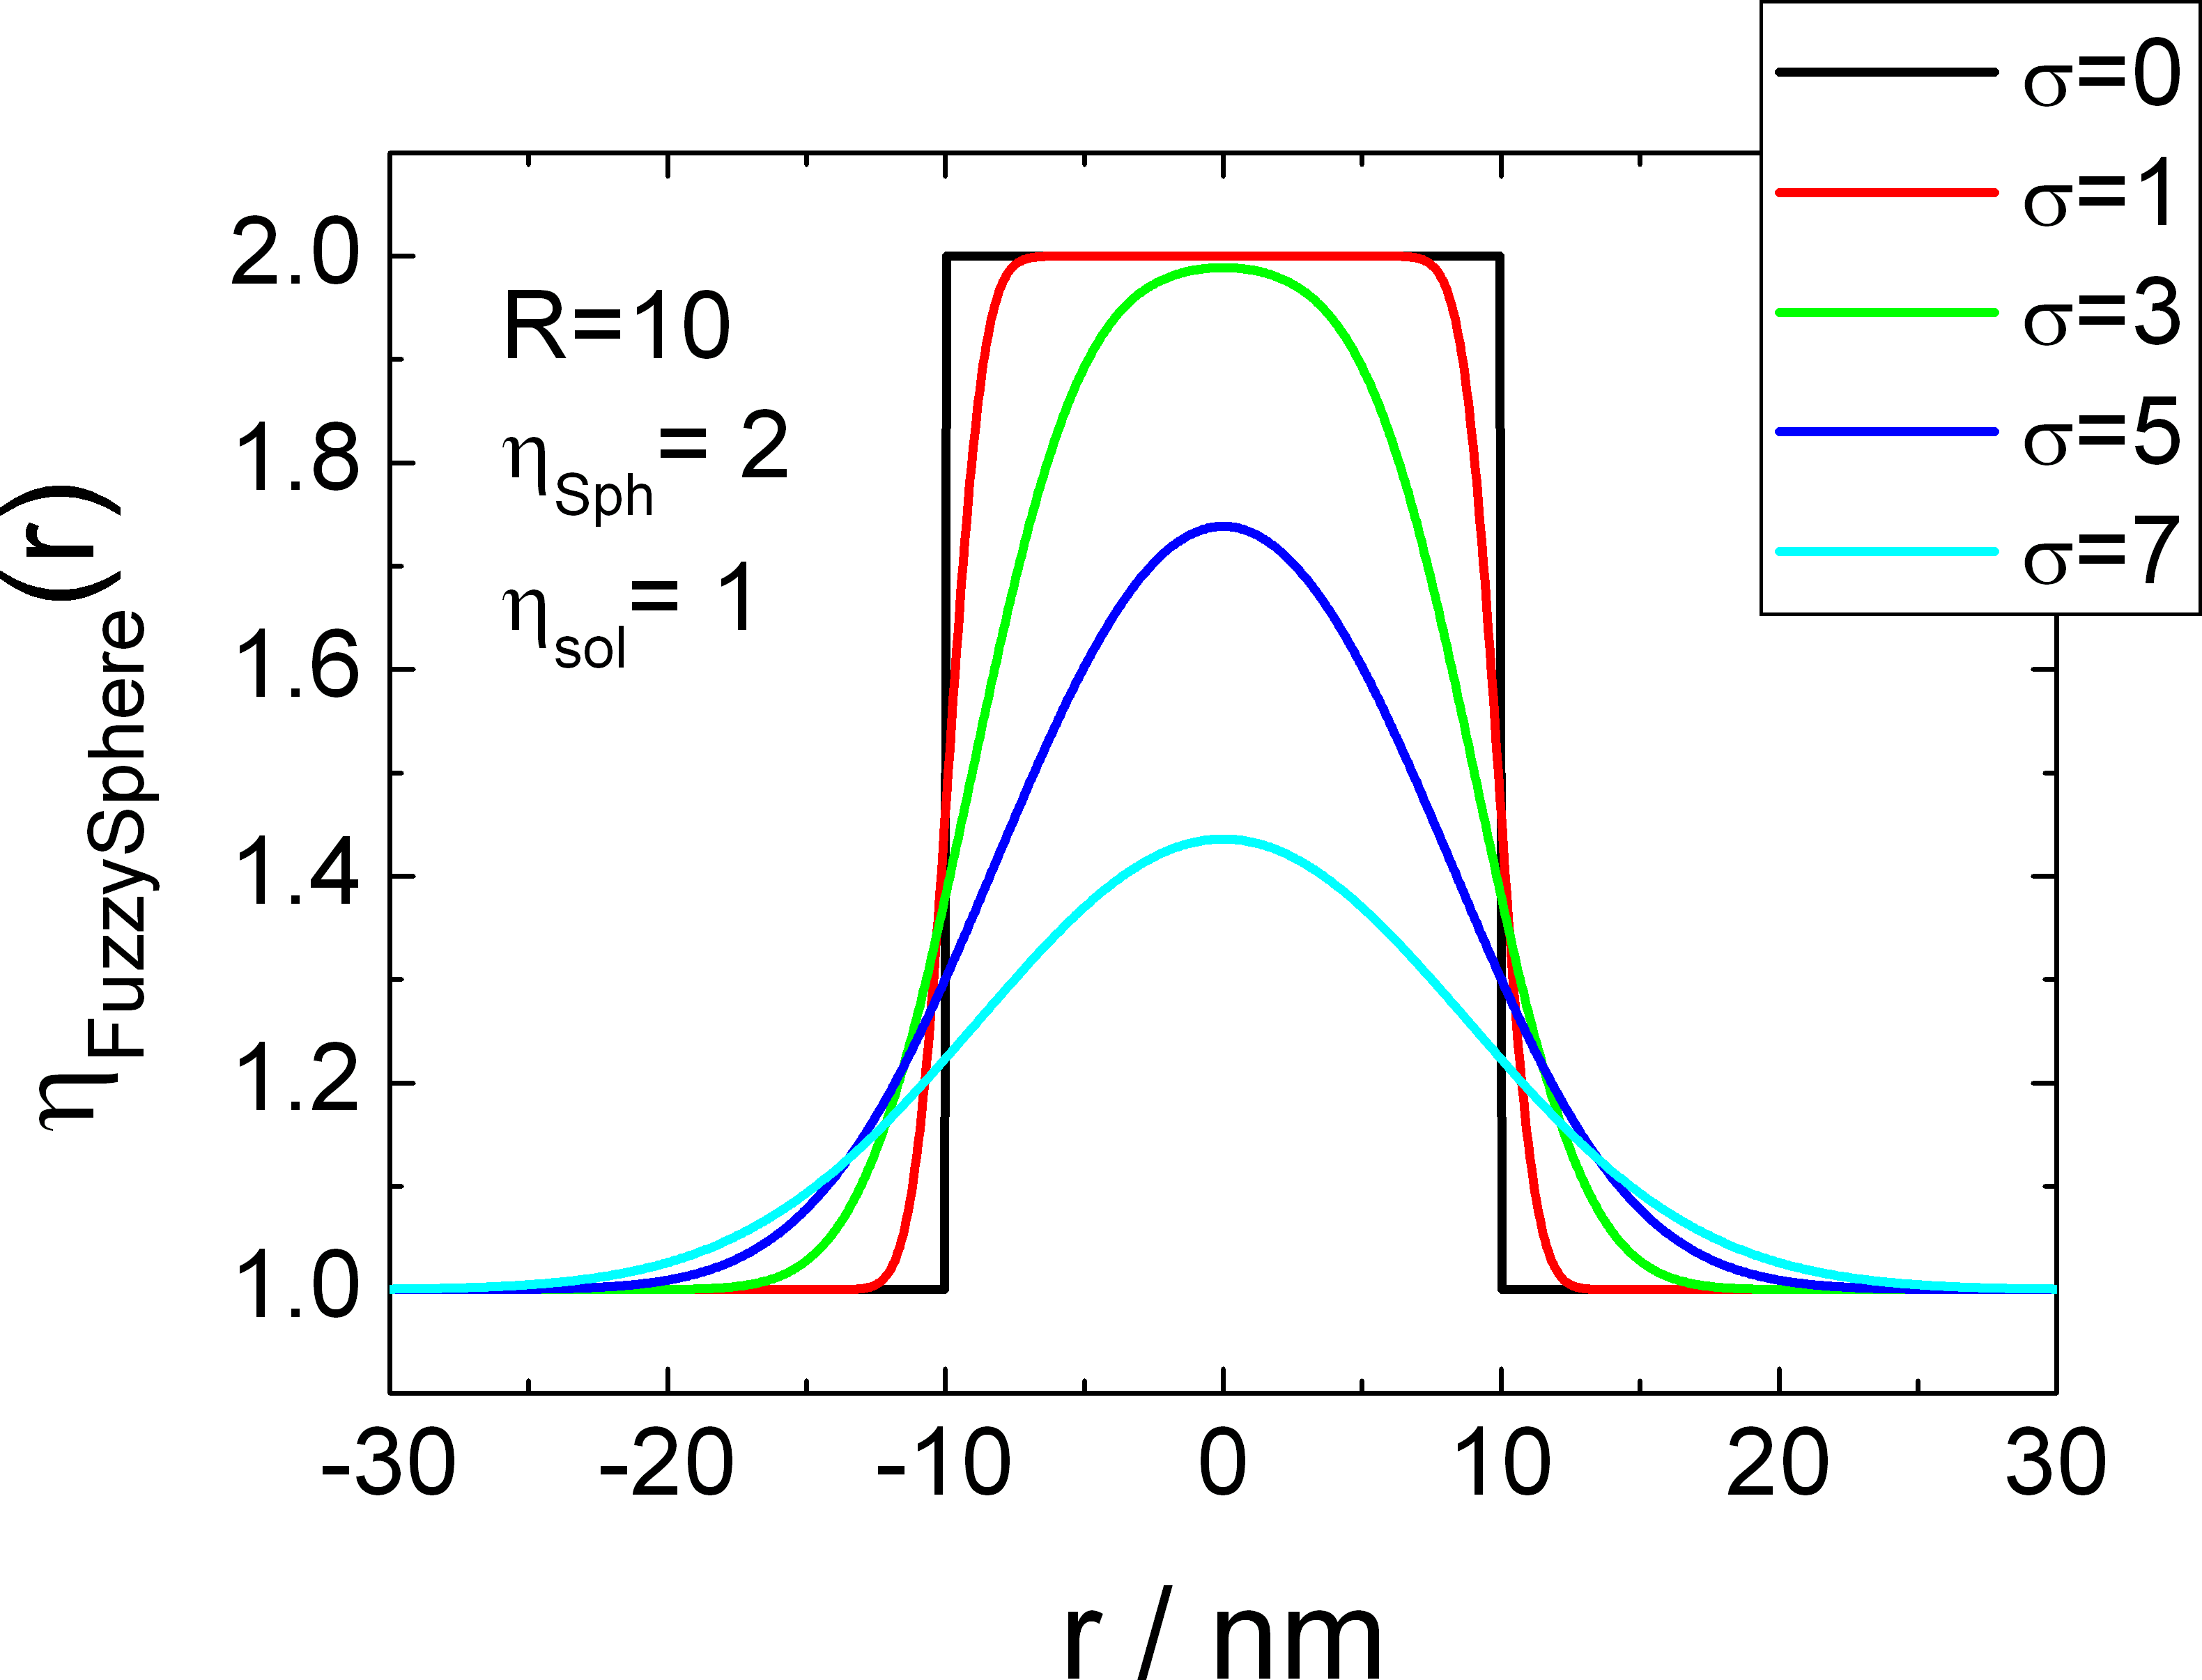
\includegraphics[width=0.7\textwidth,height=0.5\textwidth]{../images/form_factor/FuzzySphere/FuzzySphereProfile.png}
\end{center}
\caption{radial profile of a fuzzy sphere model}
\label{profile:fuzzysphere}
\end{figure}

This model can be used to calculate the scattering from spherical
particles with a "fuzzy" interface \cite{Stieger2004}. The fuzzy
interface is obtained by convoluting the radial profile of a hard
sphere with a Gaussian function.
\begin{align}
\eta_\text{FuzzySph}\left(\abs{\mathbf{r}}\right)
        &= \left(\eta_\text{HS}\star\eta_\text{Gauss}\right)(\mathbf{r}) \nonumber \\
        &= \int_{\mathbb{R}^3}\eta_\text{HS}(\boldsymbol{\tau}) \eta_\text{Gauss}(\mathbf{r}-\boldsymbol{\tau}) d\boldsymbol{\tau}
\end{align}
with
\begin{subequations}
\begin{align}
\eta_\text{HS}(\mathbf{r}) &=
\begin{cases}
\left(\eta_\text{sph}-\eta_\text{sol}\right) & \mbox{for~} \abs{\mathbf{r}}\leq R \\
0 & \mbox{for~} \abs{\mathbf{r}}>R
\end{cases} \\
\eta_\text{Gauss}(r) &= \frac{1}{2 \sqrt{2} \pi^{3/2}
\abs{\sigma}^3} \exp\left[ -\frac{\abs{\mathbf{r}}^2}{2
\abs{\sigma}^2}\right]
\end{align}
\end{subequations}
The convolution has to be done in $\mathbb{R}^3$. As the hard
sphere and Gaussian functions are radial symmetric also the
profile of the fuzzy sphere only depends on $\abs{\mathbf{r}}$. By
defining the interface via a convolution the form factor can be
easily calculated because the Fourier transform of a convolution
is the pointwise product of the Fourier transforms according to
the convolution theorem, i.e.
\begin{equation}
\begin{split}
F(Q) &= \mathcal{F}\left[\eta_\text{FuzzySph}(r) \right] \\
&=
  \mathcal{F}\left[\left(\eta_\text{HS}\star\eta_\text{Gauss}\right)(r)\right]
= \mathcal{F}\left[\eta_\text{HS}(r)\right] \mathcal{F}\left[\eta_\text{Gauss}(r)\right] \\
%&= \int_0^{\infty} \eta_\text{FuzzySph}(r)\; 4\pi r^2\frac{\sin\left(Qr\right)}{Qr} \; dr \\
&=
   \int_0^{\infty} \eta_\text{HS}(r)\; 4\pi r^2\frac{\sin\left(Qr\right)}{Qr} \; dr \int_0^{\infty} \eta_\text{Gauss}(r)\; 4\pi r^2\frac{\sin\left(Qr\right)}{Qr} \; dr \\
&= \left(\eta_\text{sph}-\eta_\text{sol}\right) 4\pi R^3%8\sqrt{2}\pi^{5/2} R^3
   \frac{\sin\left(QR\right)-QR\cos\left(QR\right)}{\left(QR\right)^3} \quad e^{\left[-\frac{1}{2}\sigma^2Q^2\right]}
\end{split}
\end{equation}

Instead of calculating the convolution integral one also can get
the radial profile of the fuzzy interface by the inverse Fourier
transformation of the scattering amplitude
\begin{align}
\eta_\text{FuzzySph}(r) &= \int_0^{\infty}
\frac{1}{\left(2\pi\right)^3} F(Q) 4\pi Q^2 dQ
\end{align}
\begin{multline}
\eta_\text{FuzzySph}(r) = \left(\eta_\text{sph}-\eta_\text{sol}\right) \\
\left( \frac{
    \left(
          e^{-\frac{\left(r + R\right)^2}{2 \sigma^2}}
        - e^{-\frac{\left(r - R\right)^2}{2 \sigma^2}}
    \right) \sigma}{\sqrt{2 \pi} r}
 + \frac{1}{2} \text{erf}\left[\frac{r + R}{\sqrt{2} \abs{\sigma}}\right]
 - \frac{1}{2} \text{erf}\left[\frac{r - R}{\sqrt{2} \abs{\sigma}}\right]
\right)
\end{multline}

Finally the scattering intensity is given by
\begin{multline}
I_\text{FuzzySph}(Q) = F^2(Q) = \\
\left[ \left(\eta_\text{sph}-\eta_\text{sol}\right) 4\pi R^3
   \frac{\sin\left(QR\right)-QR\cos\left(QR\right)}{\left(QR\right)^3} \quad e^{\left[-\frac{1}{2}\sigma^2Q^2\right]}
\right]^2
\end{multline}

The intensity $I_\text{FuzzySph}(Q)$ and also the scattering
length profile $\eta_\text{FuzzySph}(r)$ are normalized so that
\begin{align*}
 \lim_{Q \to \infty} I_\text{FuzzySph}(Q) &= \left( \frac{4}{3}\pi R^3\right)^2 \\
 \int_0^{\infty} 4\pi r^2 \; \eta_\text{FuzzySph}(r) \; \mathrm{d}r &=\frac{4}{3}\pi R^3
\end{align*}

\begin{align}
R &=\text{radius of the fuzzy sphere} \nonumber\\
\sigma &=\text{thickness of the fuzzy shell} \nonumber\\
\eta_\text{sph}   & : \text{scattering length density of sphere} \nonumber \\
\eta_\text{sol}   & : \text{scattering length density of the solvent} \nonumber \\
%I_\text{fluct}    & : \text{forward scattering of the internal fluctuation contribution} \nonumber \\
%\xi               & : \text{correlation length of the fluctuations} \nonumber
\end{align}


\vspace{5mm}

\hspace{1pt}\\
\underline{Input Parameters for model \texttt{FuzzySphere}:}\\
\begin{description}
\item[\texttt{R}] radius of the fuzzy sphere  $R$
\item[\texttt{sigma}] thickness of the fuzzy shell $\sigma$
\item[\texttt{eta\_sph}] scattering length density of sphere
$\eta_\text{sph}$ \item[\texttt{eta\_sol}] scattering length
density of solvent $\eta_\text{sol}$
%\item[\texttt{I\_fluct}] forward scattering of the internal fluctuation contribution $I_\text{fluct}$
%\item[\texttt{xi}] correlation length of the fluctuations $\xi$
\end{description}

\noindent\underline{Note:}
\begin{itemize}
\item This form factor is only defined for positive radii $R>0$.
\item For $\sigma = 0$ the limiting case of a simple hard sphere
form factor is used. \item In addition, scattering contributions
arising from fluctuations of the microgel network are often
included in this model expression as a Lorentzian function
\begin{align}
I_\text{fluct}(Q) &= \frac{I_\text{fluct}(0)}{1+\xi^2Q^2}
\end{align}
so that
\begin{align}
I(Q) &= I_\text{FuzzySph}(Q)+I_\text{fluct}(Q)
\end{align}
where $I_\text{fluct}(0)$ is the $Q=0$ limiting intensity and
$\xi$ represents the correlation length of the fluctuations, which
can be considered to be related to the blob or mesh size. It
should be noted that the Lorentzian describes the ensemble average
correlations in the polymer network.

\end{itemize}

\begin{figure}[htb]
\begin{center}
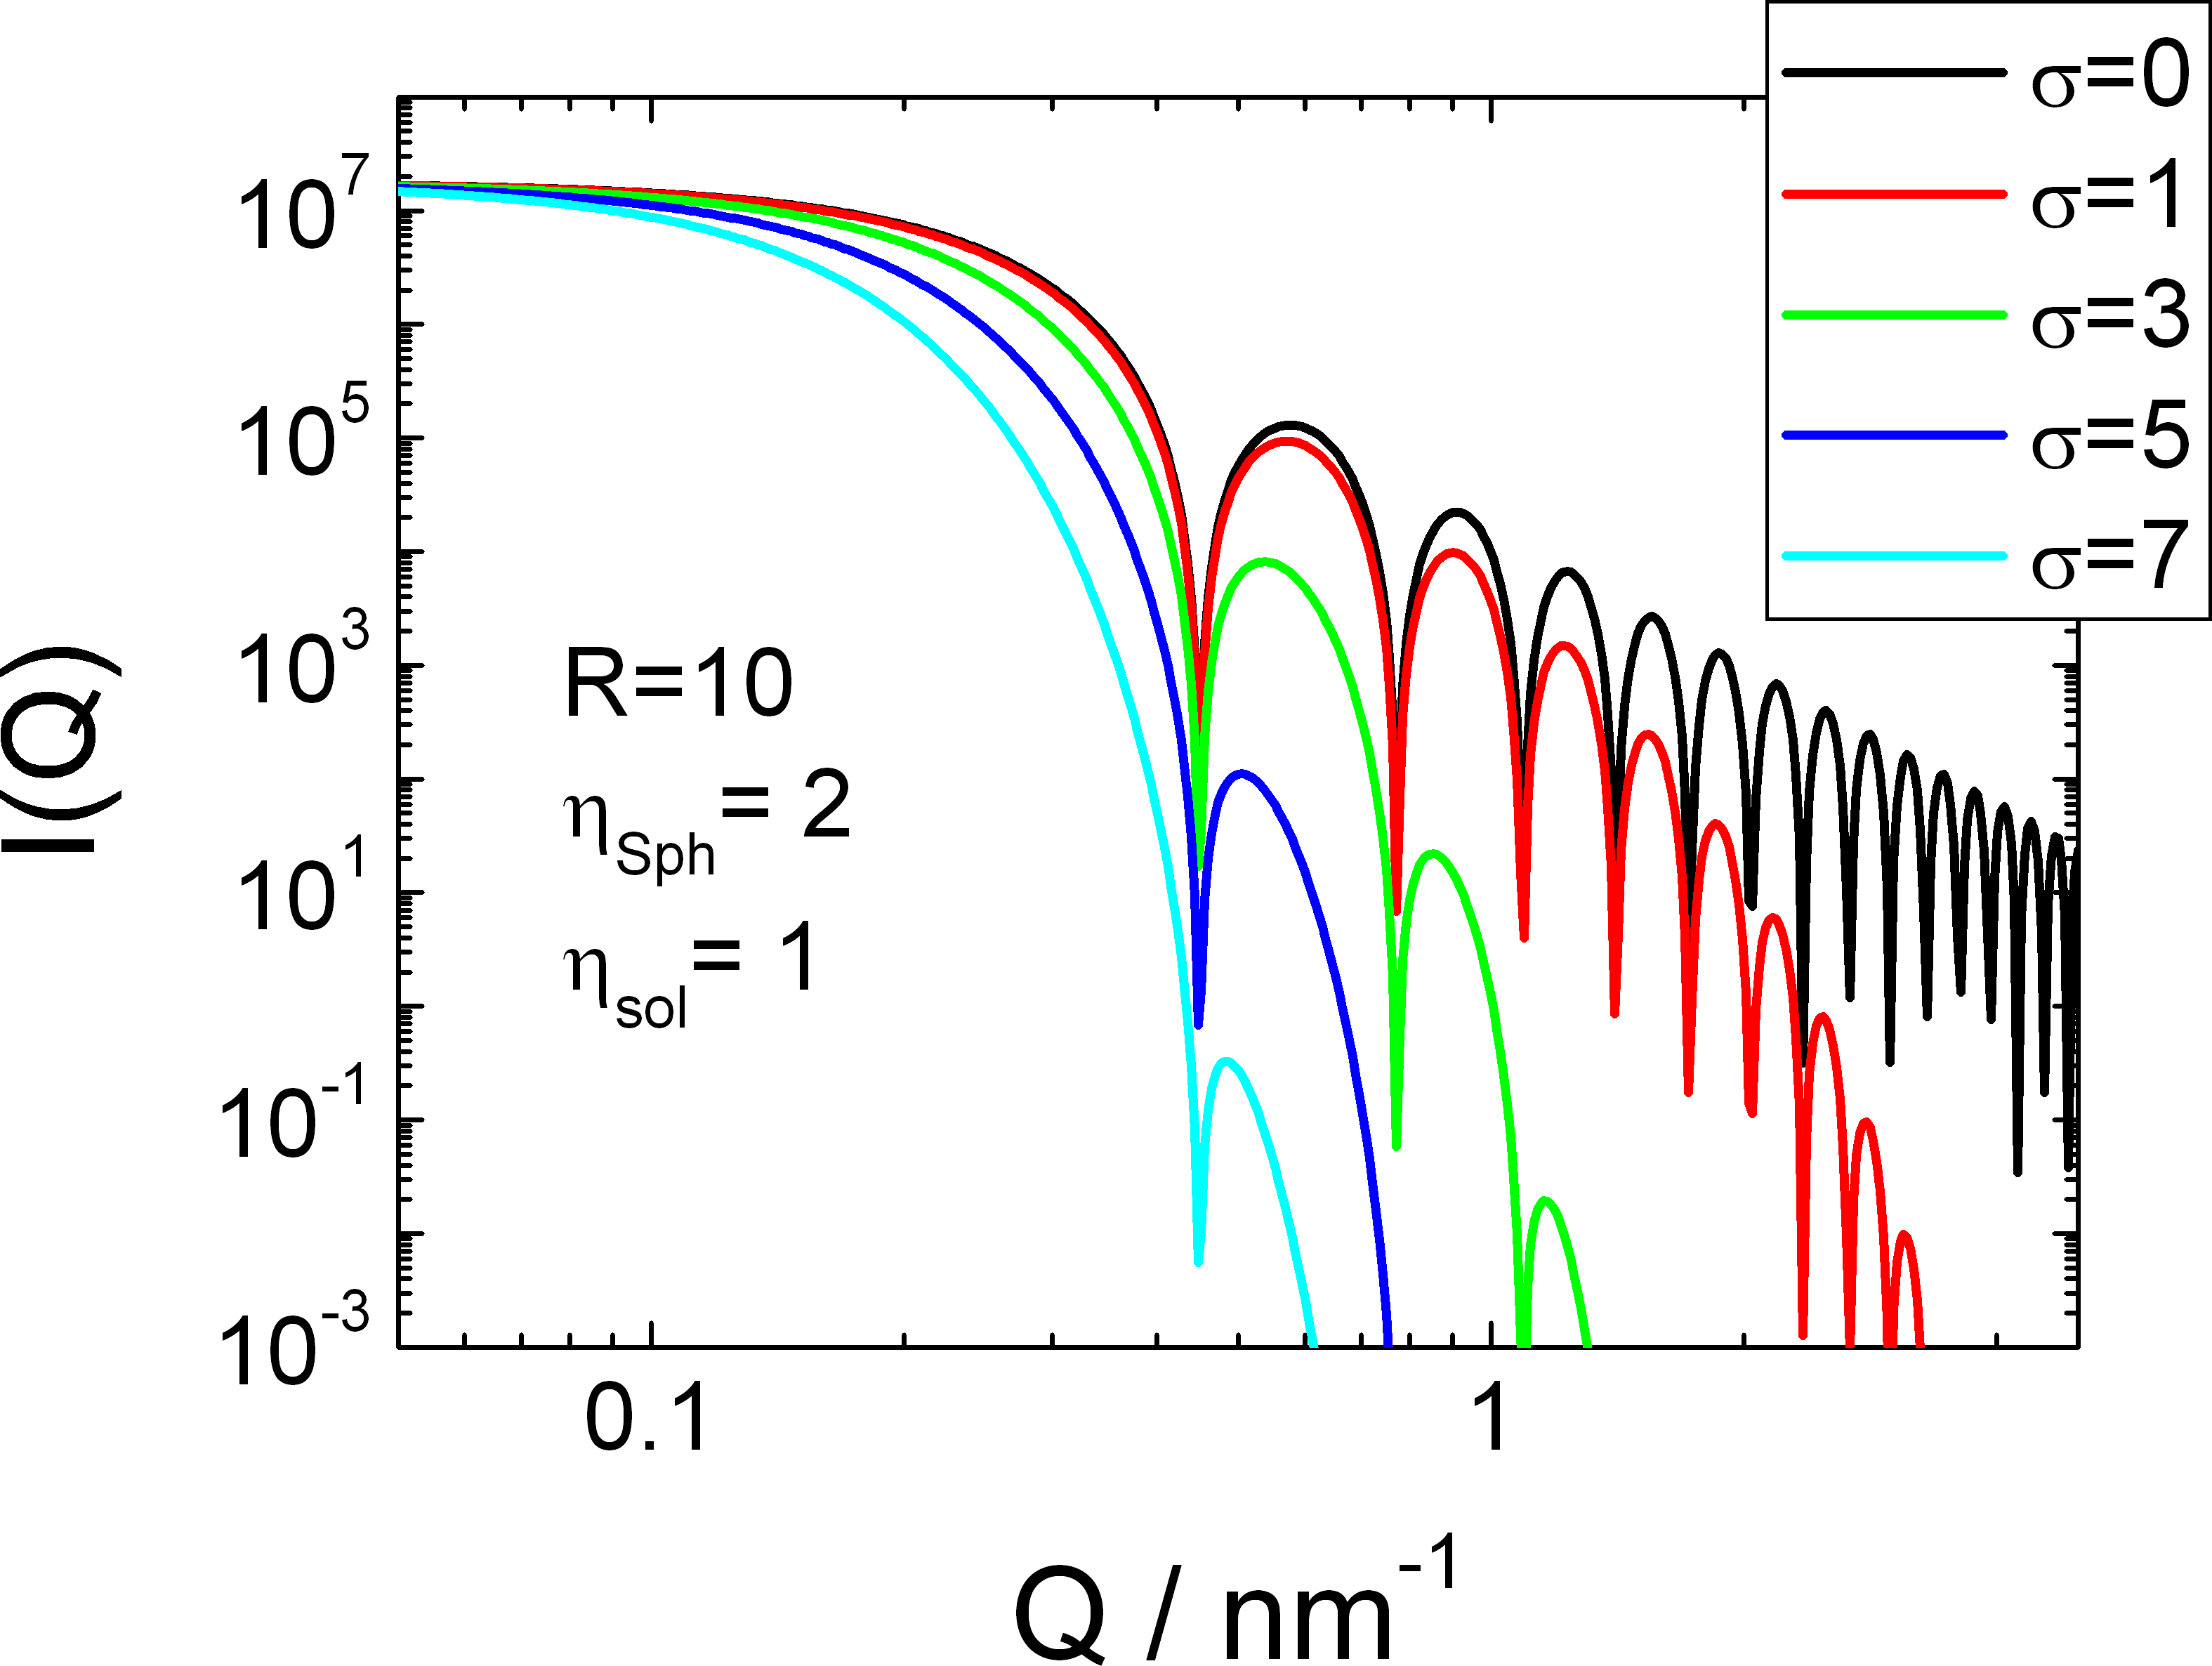
\includegraphics[width=0.7\textwidth,height=0.5\textwidth]{../images/form_factor/FuzzySphere/FuzzySphereIQ.png}
\end{center}
\caption{Scattering intensity of a fuzzy sphere. The scattering
intensity has been calculated for a core radius $R=10$, a
scattering length density of the FuzzySphere of
$\eta_\text{Sph}=1$, a scattering length density of the solvent
$\eta_\text{sol}=1$, and several widths of the "fuzzy" shell}
\label{fig:I_FuzzySphere}
\end{figure}


%%%%%%%%%%%%%%%%%%%%%%%%%%%%%%%%%%%%%%%%%%%%%%%%%%%%%%%%%%%%%%%%%%%%%%%%%%%%%%%%%%%%%%%%
\clearpage
\section{Ferrofluids} \hspace{1pt}
\label{sec:ferrofluid}

%%%%%%%%%%%%%%%%%%%%%%%%%%%%%%%%%%%%%%%%%%%%%%%%%%%%%%%%%%%%%%%%%%%%%%%%%%%%%%%%%%%%%%%%
\clearpage
\section{LogNorm\_fp} \hspace{1pt}
\label{sec:sd_lognorm_fp}

The \texttt{LogNorm} distribution is a continuous distribuion in which the logarithm of a variable
has a normal distribution.
\begin{subequations}
\begin{align}
\text{LogNorm}(x,N,\sigma,p,\mu) &=  \frac{N}{c_\text{LN}}
                                    \frac{1}{x^{p}}\,
                                    \exp\!\!\left(-\frac{\ln(x/\mu)^2}{2\sigma^2}\right) \\
c_\text{LN} &= \sqrt{2\pi}\,\sigma \,\mu^{1-p}
\,\exp\!\!\left((1-p)^2\frac{\sigma^2}{2}\right)
\label{eq:LogNorm}
\end{align}
\end{subequations}
where $\sigma$ is the width parameter, $p$ a shape parameter, $\mu$ is the location parameter.
$c_\text{LN}$ is choosen so that $\int_0^\infty\! \text{LogNorm}(x,\mu,\sigma,p)\,dR = N$
The mode of the distribution is defined as
\begin{align}
x_\text{mode} = \mu e^{-p \sigma^2}
\end{align}
and the $n^\text{th}$ moment $\langle X^n\rangle$ of the \texttt{LogNorm} distribution as
\begin{align}
\langle X^n\rangle = \frac{\int X^n\, \textrm{LogNorm}(X)\, dX}{\int \textrm{LogNorm}(X)\, dX} =
\mu^n \, e^{\frac{1}{2} \sigma^2 n (2 - 2 p + n)}.
\label{eq:nMoment:LogNorm}
\end{align}

Instead of using the parameter $N$ (particle number density) another
Log-Normal size distribution namely {\tt LogNorm\_fp} with the
volume fraction $f_p$ as a parameter has been implemented.
Using the volume fraction as a scaling parameter requires that the intensity is
given in units of cm$^{-1}$ and the scattering vector in nm$^{-1}$. Furthermore
the scattering contrast needs to be supplied in units of cm$^{-2}$. More details
about absolute intensity can be found in chapter \ref{ch:absint}.
The volume fraction $f_p$ can be obtained from the \texttt{LogNorm}-distribution
(eq.\ \ref{eq:LogNorm}) by integrating over the particle volume $V_P$. In case
of spheres we get
\begin{align}
f_p &= 10^{21} \int_0^\infty \mathrm{LogNorm}(R,N,\sigma,p,\mu) V_P(R) \, dR \label{eq:fpMomentsV} \\
    &= 10^{21} \int_0^\infty \mathrm{LogNorm}(R,N,\sigma,p,\mu) \frac{4}{3}\pi R^3 \, dR = 10^{21}
    N \frac{4}{3}\pi \langle X^3 \rangle .
\end{align}
The scaling factor $10^{21}$ depends on the actual units. More details are
given in section \ref{sec:volumefraction}.


For other shapes than spheres the corresponding volume of the object has to be used in eq.\ \ref{eq:fpMomentsV}.
In case of cylinders the volume is given by $V_\text{cyl}=\pi R^2 L$. Depending whether the radius $R$ or the
cylinder length $L$ has a size distribution the volume fraction $f_p$ is calculated differently namely
in case for a radius distribution by
\begin{align}
f_p &= 10^{21} \int_0^\infty \mathrm{LogNorm}(R) V_\text{cyl}(R,L) \, dR \label{eq:fpMomentsV} \\
    &= 10^{21} \int_0^\infty \mathrm{LogNorm}(R) \pi R^2L \, dR = 10^{21} N \pi L \langle X^2 \rangle
\end{align}
and in case of a length distribution by
\begin{align}
f_p % &= 10^{21} \int_0^\infty \mathrm{LogNorm}(L) V_\text{cyl}(R,L) \, dL  \\
    &= 10^{21} \int_0^\infty \mathrm{LogNorm}(L) \pi R^2L \, dL = 10^{21} N \pi R^2 \langle X \rangle .
\end{align}
As the cylinder volume depends on $R^2$  and $L$ either the second or the first moment of the distribution
function is involved in calculating the volume fraction depending which parameter has a distribution.
For a spherical shell a sum of different moments has to be used as listed in table \ref{tab:volumefraction}.

\begin{table}
  \centering
  \scriptsize
\rotatebox{270}{
  \setlength\doublerulesep{0pt}
\begin{tabular}{|>{\columncolor[gray]{1.0}[0.8\tabcolsep][0.8\tabcolsep]} c%
                |>{\columncolor[gray]{1.0}[0.8\tabcolsep][0.8\tabcolsep]} l%
                |>{\columncolor[gray]{1.0}[0.8\tabcolsep][0.8\tabcolsep]} c%
                |>{\columncolor[gray]{1.0}[0.8\tabcolsep][0.8\tabcolsep]} c%
                |>{\columncolor[gray]{1.0}[0.8\tabcolsep][0.8\tabcolsep]} c%
                |>{\columncolor[gray]{1.0}[0.8\tabcolsep][0.8\tabcolsep]} c%
                |>{\columncolor[gray]{1.0}[0.8\tabcolsep][0.8\tabcolsep]} c%
                |>{\columncolor[gray]{1.0}[0.8\tabcolsep][0.8\tabcolsep]} c|}
 \rowcolor[gray]{0.7}
 shape &  form factor &  distrib. & \texttt{length2} & \texttt{length3}
                             &  volume  & $V$ & $N(f_p)$\\
 \rowcolor[gray]{0.7}
  & &  param.\ & & & & &  \\
  \hline\hline
1      &  \texttt{Sphere} & $R$  & not used & not used & whole sph. &
            \mbox{\tiny$\frac{4}{3}\pi R^3$} &
            $  \frac{f_p}{10^{21}} \frac{3}{4\pi} \, \frac{1}{\langle X^3 \rangle}$ \\
 \rowcolor[gray]{0.95}
2 &  \texttt{Cylinder}    & $R$  & $L$ & not used & whole cyl. &
            \mbox{\tiny$ \pi R^2 L$} &
            $  \frac{f_p}{10^{21}} \frac{1}{\pi} \, \frac{1}{\langle X^2 \rangle L}$ \\
 \rowcolor[gray]{0.95}
3 &  \texttt{Cylinder}   & $L$   & $R$ & not used & whole cyl. &
            \mbox{\tiny$\pi R^2 L$} &
            $  \frac{f_p}{10^{21}} \frac{1}{\pi} \, \frac{1}{R^2 \langle X^1 \rangle}$ \\
4 &  \texttt{Sph.Sh.iii}    & $R$ & $\Delta R$ & not used & core+shell&
            \mbox{\tiny$ 4\pi \left(R^2 \Delta R +R \Delta R^2+\frac{1}{3}\Delta R^3+\frac{1}{3} R^3\right)$} &
            $  \frac{f_p}{10^{21}} \frac{1}{4\pi}\,
            \frac{1}{
            \frac{1}{3}\langle X^3 \rangle +
            \langle X^2 \rangle \Delta R+
            \langle X^1 \rangle \Delta R^2+
            \langle X^0 \rangle \frac{\Delta R^3}{3}}$\\
5 &  \texttt{Sph.Sh.iii}    & $\Delta R$ & $R$ & not used & core+shell &
            \mbox{\tiny$ 4\pi \left(R^2 \Delta R +R \Delta R^2+\frac{1}{3}\Delta R^3+\frac{1}{3} R^3\right)$} &
            $  \frac{f_p}{10^{21}} \frac{1}{4\pi}\,
            \frac{1}{
            \frac{1}{3}R^3\langle X^0\rangle +
            R^2 \langle X^1 \rangle+
            R \langle X^2 \rangle +
            \frac{1}{3}\langle X^3 \rangle}$ \\
 \rowcolor[gray]{0.95}
6 &  \texttt{Sph.Sh.iii}    & $R$ & $\Delta R$ & not used & core &
            \mbox{\tiny$ \frac{4}{3}\pi R^3$} &
            $  \frac{f_p}{10^{21}} \frac{3}{4\pi} \, \frac{1}{\langle X^3 \rangle}$\\
 \rowcolor[gray]{0.95}
7 &  \texttt{Sph.Sh.iii}    & $\Delta R$ & $R$ & not used & core &
            \mbox{\tiny$ \frac{4}{3}\pi R^3$} &
            $  \frac{f_p}{10^{21}} \frac{3}{4\pi} \, \frac{1}{R^3 \langle X^0 \rangle}$\\
8 &  \texttt{Sph.Sh.iii}    & $R$ & $\Delta R$ & not used & shell &
            \mbox{\tiny$ 4\pi \left(R^2 \Delta R +R \Delta R^2+\frac{1}{3}\Delta R^3\right)$} &
            $  \frac{f_p}{10^{21}} \frac{1}{4\pi}\,
            \frac{1}{\langle X^2 \rangle \Delta R+
            \langle X^1 \rangle \Delta R^2+
            \langle X^0 \rangle \frac{\Delta R^3}{3}}$ \\
9 &  \texttt{Sph.Sh.iii}    & $\Delta R$ & $R$ & not used & shell &
            \mbox{\tiny$ 4\pi \left(R^2 \Delta R +R \Delta R^2+\frac{1}{3}\Delta R^3\right)$} &
            $  \frac{f_p}{10^{21}} \frac{1}{4\pi}\,
            \frac{1}{R^2 \langle X^1 \rangle+
            R \langle X^2 \rangle +
            \frac{1}{3}\langle X^3 \rangle}$ \\
 \rowcolor[gray]{0.95}
10 &  \texttt{CylShell1}    & $R$ & $\Delta R$ & $L$ & core+shell &
            \mbox{\tiny$ \pi L\left( \Delta R^2 + 2R \Delta R +R^2\right)$} &
            $  \frac{f_p}{10^{21}} \frac{1}{\pi}\,
            \frac{1}{
            L\left( \Delta R^2 \langle X^0 \rangle + 2\langle X^1 \rangle \Delta R +\langle X^2 \rangle\right)
            }$ \\
 \rowcolor[gray]{0.95}
11 &  \texttt{CylShell1}    & $\Delta R$ & $R$ & $L$ &  core+shell  &
            \mbox{\tiny$ \pi L\left( \Delta R^2 + 2R \Delta R +R^2\right)$} &
            $  \frac{f_p}{10^{21}} \frac{1}{\pi}\,
            \frac{1}{
            L\left( \langle X^2 \rangle + 2R \langle X^1 \rangle +R^2\langle X^0 \rangle\right)
            }$\\
 \rowcolor[gray]{0.95}
12 &  \texttt{CylShell1}    & $L$ & $R$ & $\Delta R$ &  core+shell  &
            \mbox{\tiny$ \pi L\left( \Delta R^2 + 2R \Delta R +R^2\right)$} &
            $  \frac{f_p}{10^{21}} \frac{1}{\pi}\,
            \frac{1}{
            \langle X^1 \rangle \left( \Delta R^2 + 2R \Delta R +R^2\right)
            }$\\
13 &  \texttt{CylShell1}    & $R$ & $\Delta R$ & $L$ & core&
            \mbox{\tiny$ \pi L R^2$} &
            $  \frac{f_p}{10^{21}} \frac{1}{\pi} \, \frac{1}{\langle X^2 \rangle L}$ \\
14 &  \texttt{CylShell1}    & $\Delta R$ & $R$ & $L$ &  core  &
            \mbox{\tiny$ \pi L R^2$} &
            $  \frac{f_p}{10^{21}} \frac{1}{\pi} \, \frac{1}{R^2 L \langle X^0 \rangle}$\\
15 &  \texttt{CylShell1}    & $L$ & $R$ & $\Delta R$ &  core  &
            \mbox{\tiny$ \pi L R^2$} &
            $  \frac{f_p}{10^{21}} \frac{1}{\pi} \, \frac{1}{R^2 \langle X^1 \rangle}$\\
 \rowcolor[gray]{0.95}
16 &  \texttt{CylShell1}    & $R$ & $\Delta R$ & $L$ & shell  &
            \mbox{\tiny$ \pi L\left( \Delta R^2 + 2R \Delta R\right)$} &
            $  \frac{f_p}{10^{21}} \frac{1}{\pi} \,
            \frac{1}{L\left( \Delta R^2\langle X^0 \rangle + 2\langle X^1 \rangle \Delta R\right)}$  \\
 \rowcolor[gray]{0.95}
17 &  \texttt{CylShell1}    & $\Delta R$ & $R$ & $L$ &  shell  &
            \mbox{\tiny$ \pi L\left( \Delta R^2 + 2R \Delta R\right)$} &
            $  \frac{f_p}{10^{21}} \frac{1}{\pi} \,
            \frac{1}{L\left( \langle X^2 \rangle + 2R \langle X^1 \rangle\right)}$  \\
 \rowcolor[gray]{0.95}
18 &  \texttt{CylShell1}    & $L$ & $R$ & $\Delta R$ &  shell  &
            \mbox{\tiny$ \pi L\left( \Delta R^2 + 2R \Delta R\right)$} &
            $  \frac{f_p}{10^{21}} \frac{1}{\pi} \,
            \frac{1}{\langle X^1 \rangle\left( \Delta R^2 + 2R \Delta R\right)}$  \\
\hline
\end{tabular}
}

\vspace{3mm}

  \caption{The number density $N$ expressed in terms of volume fraction $f_p$ and moments
  $\langle X^n\rangle$ of the distribution function for
  some particle shapes and different parameters having a distribution.
 The factor $10^{21}$ is needed due to unit
conversion. It is assumed that the radius is given in nm, the
intensity in cm$^{-1}$ and the scattering length densities in
cm$^{-2}$.}
\label{tab:volumefraction}
\end{table}
